\documentclass[11pt]{article}
% Shared preamble for the research-note series.
% Create note-specific content in the per-note directory; keep common macros here.
\usepackage[margin=1in]{geometry}
\usepackage[T1]{fontenc}
\usepackage[utf8]{inputenc}
\usepackage{amsmath,amssymb}
\usepackage{booktabs,longtable,array}
\usepackage{graphicx}
\usepackage{float}
\usepackage{enumitem}
\usepackage{xcolor}
\usepackage{hyperref}
\usepackage{caption}
\usepackage{titlesec}
\hypersetup{colorlinks=true, linkcolor=blue!60!black, urlcolor=blue!60!black, citecolor=blue!60!black}
\setlist[itemize]{leftmargin=1.25em, itemsep=0.2em, topsep=0.3em}
\setlist[enumerate]{leftmargin=1.4em, itemsep=0.2em, topsep=0.3em}
\setlength{\parindent}{0pt}
\setlength{\parskip}{0.6em}
\newcommand{\statusbox}[2]{%
  \noindent\fcolorbox{black}{gray!10}{%
    \parbox{\dimexpr\linewidth-2\fboxsep-2\fboxrule\relax}{%
      \textbf{Status:} #1\\#2
    }%
  }
}

% Shared notation helpers for the research-note series.
\newcommand{\Jlin}{J}
\newcommand{\Jphys}{J_{\mathrm{phys}}}
\newcommand{\Jsurf}{J_{\mathrm{surf}}}
\newcommand{\JdB}{J_{\mathrm{dB}}}
\newcommand{\phiopt}{\phi_{\mathrm{opt}}}
\newcommand{\sigmathreedb}{\sigma_{3\mathrm{dB}}}
\newcommand{\Nt}{N_t}
\newcommand{\Nphi}{N_{\phi}}
\newcommand{\Lfiber}{L}
\newcommand{\Pcont}{P}
\newcommand{\band}{\mathcal{B}_{\mathrm{Raman}}}
\newcommand{\todoitem}[1]{\textcolor{red!70!black}{\textbf{TODO:} #1}}


\usepackage{tabularx}
\usepackage{placeins}

\title{Multimode Raman Baselines and Cost Choice}
\author{Fiber Raman Suppression Project}
\date{Evidence snapshot: 2026-04-28}

\begin{document}
\maketitle

\begin{abstract}
This note summarizes the current multimode-fiber Raman-suppression lane. The
accepted result is a qualified simulation finding: in an idealized six-mode
GRIN-50 model, one shared spectral phase can reduce the simulated Raman-band
fraction by \(31.7\,\mathrm{dB}\) while passing corrected temporal-edge
diagnostics. The most important part of the story is that an earlier large-gain
solution was rejected after raw edge diagnostics exposed temporal-window
contamination. The current result is therefore meaningful, but not a generic
experimental claim about arbitrary multimode fibers.
\end{abstract}

\section*{Claim Status}
\statusbox{qualified simulation result}{The MMF lane is closed/exploring. It is
usable as a presentation-ready simulation result with clear claim boundaries:
shared spectral phase shaping suppresses Raman-band generation in one idealized
GRIN-50 setting under strict diagnostics. It is not yet a paper-grade or
experiment-grade universal MMF result.}

\section{Question and Thesis}

The single-mode notes optimize one spectral phase for one propagation mode. In
a multimode fiber, the field has several mode amplitudes:
\[
    \hat u_{m,k}(z),
\]
where \(m\) indexes mode and \(k\) indexes frequency. The question is:
\[
    \text{Can one shared spectral phase reduce Raman generation across a multimode field?}
\]

The current evidence says yes in a constrained simulation. The accepted case is
GRIN-50 with six scalar modes, length \(L=2\,\mathrm{m}\), power
\(P=0.20\,\mathrm{W}\), \(N_t=4096\), and a \(96\,\mathrm{ps}\) time window.
The optimized shared phase reduces the summed Raman-band objective from
\(-17.96\,\mathrm{dB}\) to \(-49.69\,\mathrm{dB}\).

\begin{figure}[H]
\centering
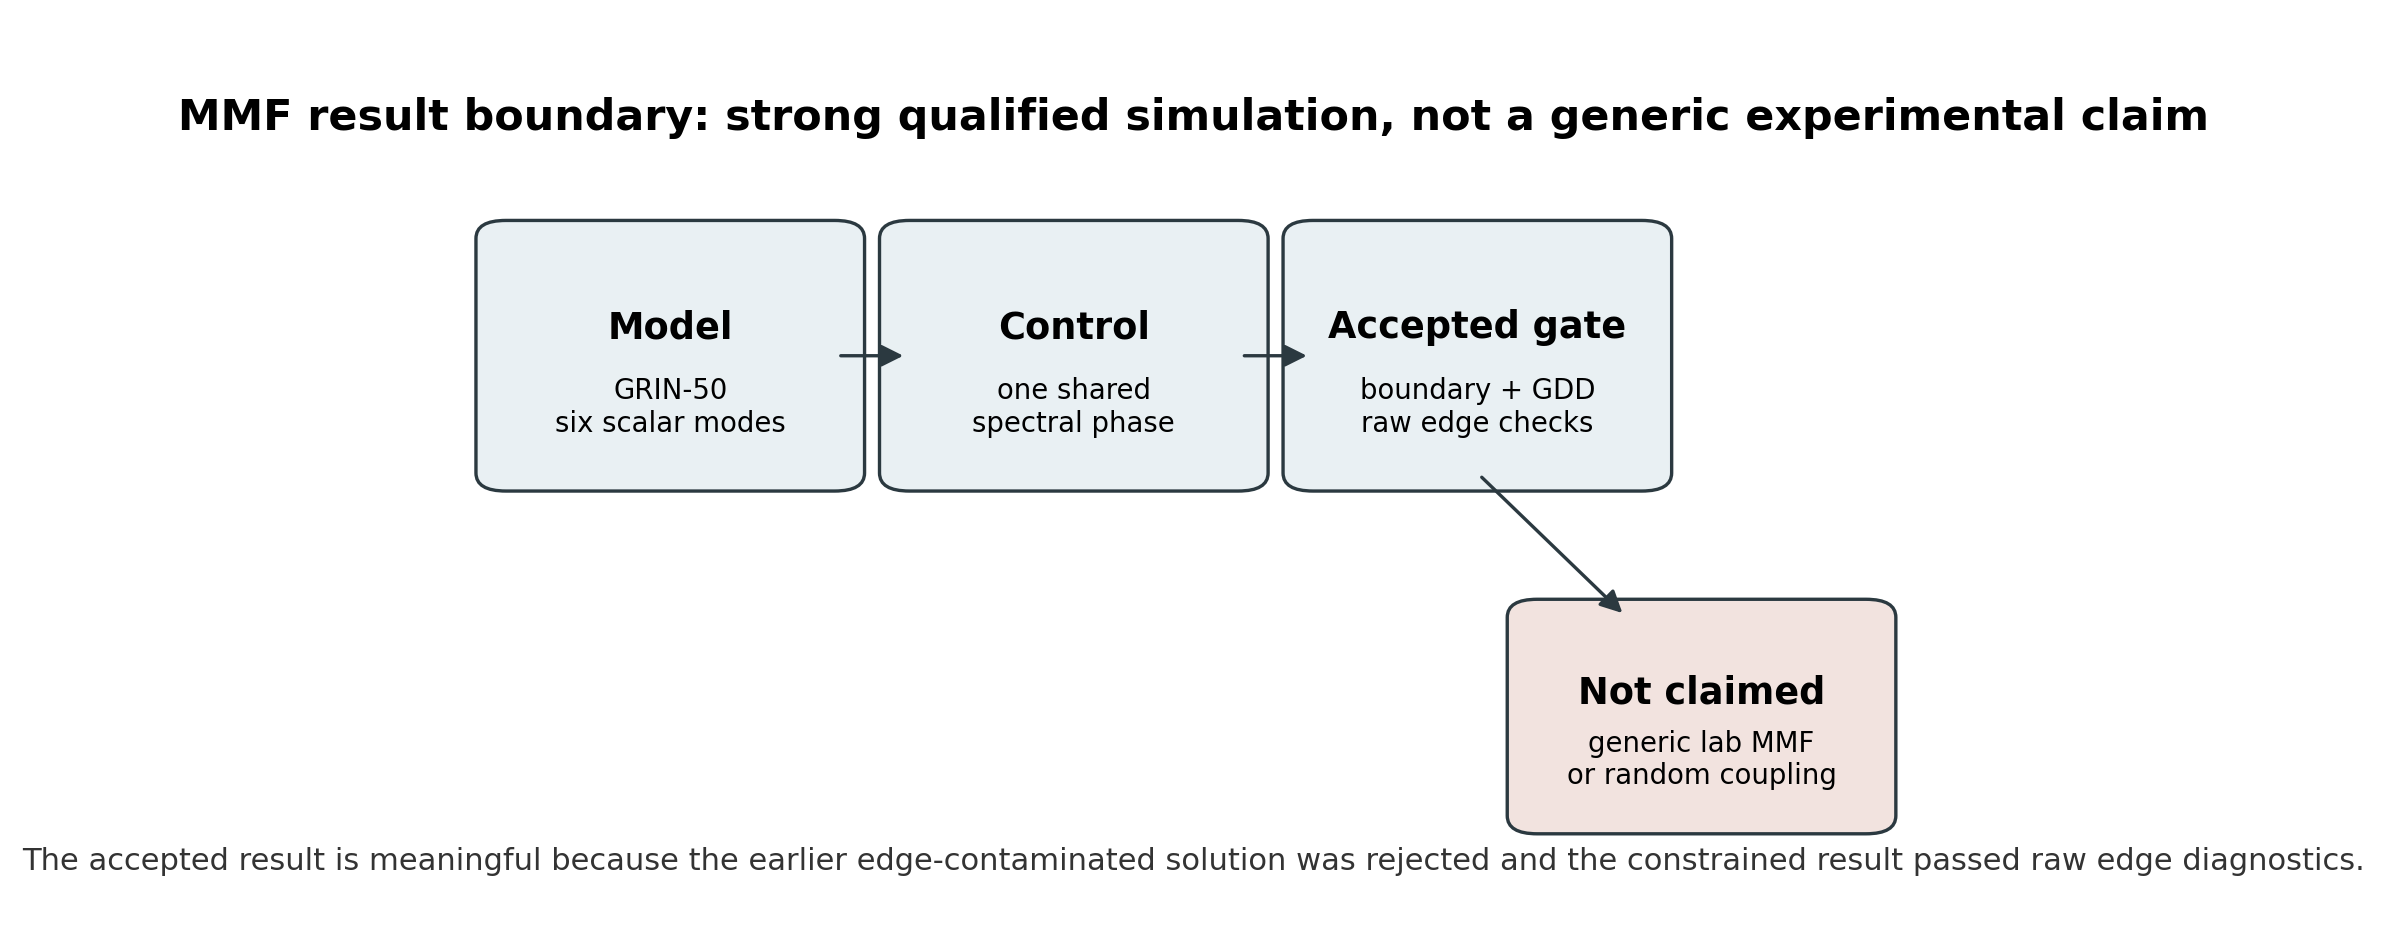
\includegraphics[width=0.95\linewidth]{figures/mmf_claim_boundary.png}
\caption{The current MMF result is intentionally narrow. The project has a
credible constrained simulation candidate, not a generic experimental claim for
all multimode fibers or all launch conditions.}
\end{figure}

\section{Why MMF Is Subtle}

Multimode fibers are not just single-mode fibers with a bigger vector. Raman
energy can appear differently by mode, launch composition matters, and mode
coupling can change the nonlinear evolution. Experiments and simulations of
graded-index multimode fibers show mode-resolved Raman cascades
\cite{pourbeyram2013}, nonlinear beam self-cleaning \cite{krupa2017}, and
launch/wavefront sensitivity \cite{deliancourt2019,sidelnikov2019}.

That literature shapes the claim boundary. A summed output spectrum is not
enough. A credible MMF result needs:
\begin{itemize}
    \item a clear objective: summed, fundamental-mode, or worst-mode Raman
    fraction;
    \item mode-resolved inspection, not only a total spectrum;
    \item temporal-window diagnostics, because pseudospectral propagation uses
    periodic time windows \cite{melchert2021};
    \item an explicit statement of launch and coupling assumptions.
\end{itemize}

\subsection*{TL;DR}

The MMF result is harder to explain because there are two kinds of structure:
frequency structure and mode structure. The shared phase only controls the
frequency structure. It does not independently control the transverse modal
wavefront, and it does not prove robustness to every possible launch.

\section{Model, Objective, and Gradients}

The accepted model is:
\[
    \text{GRIN-50},\quad M=6,\quad L=2\,\mathrm{m},\quad
    P=0.20\,\mathrm{W}.
\]
The same spectral phase is applied to all modes:
\[
    \hat u_{m,k}(0;\phi)=\hat u_{m,k,0}e^{i\phi_k}.
\]

The primary objective is the mode-summed Raman fraction:
\[
    J_{\mathrm{sum}} =
    \frac{\sum_m\sum_{k\in\band}|\hat u_{m,k}(L)|^2}
         {\sum_m\sum_k|\hat u_{m,k}(L)|^2}.
\]
The diagnostic report also computes a fundamental-mode fraction and worst-mode
fraction so the improvement cannot hide inside a summed detector. For the
accepted run:
\[
    J_{\mathrm{sum}}=-49.69\,\mathrm{dB},\qquad
    J_{\mathrm{fund}}=-49.65\,\mathrm{dB},\qquad
    J_{\mathrm{worst}}=-45.35\,\mathrm{dB}.
\]

The shared-phase gradient sums the modal sensitivities:
\[
    \frac{\partial J}{\partial \phi_k}
    =
    2\operatorname{Re}\sum_m
    \lambda_{m,k}(0)^*\, i\,\hat u_{m,k}(0).
\]
This is the same phase-chain rule as the single-mode case, except every mode
contributes to the same phase pixel.

\subsection*{Where the Shared-Phase Gradient Comes From}

Start with one frequency sample \(k\). The optimizer is not choosing a separate
phase for every mode. It chooses one number \(\phi_k\), and that same number is
applied to all modal spectra:
\[
    \hat u_{m,k}(0;\phi)=\hat u_{m,k,0}e^{i\phi_k}.
\]
A small phase change therefore gives
\[
    \delta \hat u_{m,k}(0)=i\hat u_{m,k}(0)\delta\phi_k.
\]
If \(\lambda_{m,k}(0)=\partial J/\partial \hat u_{m,k}(0)^*\) is the adjoint
sensitivity at the input, then the real objective changes by
\[
    \delta J =
    2\operatorname{Re}\sum_{m,k}
    \lambda_{m,k}(0)^*\,\delta \hat u_{m,k}(0).
\]
Substituting the phase perturbation and collecting the coefficient of
\(\delta\phi_k\) gives the formula above. The only new MMF feature is the modal
sum: all modes vote on the same phase knob.

\subsection*{TL;DR for the Board}

Think of each wavelength as one knob shared by six mode channels. Turning that
knob rotates the complex field in every mode at that wavelength. The adjoint
tells us whether each modal rotation helps or hurts the Raman objective, and
the gradient adds those six votes into one update for the shared knob.

\subsection*{Accepted Regularized Surface}

The accepted constrained run uses a dB-scaled surface of the form
\[
    10\log_{10}\left(
    J_{\mathrm{sum}}
    +\lambda_{\mathrm{gdd}}R_{\mathrm{gdd}}
    +\lambda_{\mathrm{boundary}}R_{\mathrm{boundary}}
    \right),
\]
with
\[
    \lambda_{\mathrm{gdd}}=10^{-4},
    \qquad
    \lambda_{\mathrm{boundary}}=0.05.
\]
The boundary term is central to this note because it distinguishes the rejected
result from the accepted one.

\section{Diagnostic Correction}

The earlier MMF result looked strong, but it was not accepted. The problem was
temporal-window trust. The corrected convention is:
\[
    \hat u = \mathrm{ifft}(u_t),
    \qquad
    u_t = \mathrm{fft}(\hat u).
\]
After this correction, the unregularized optimized output still had about
\(5.02\times 10^{-2}\) temporal-edge energy. That is too high, so the result
was rejected as a boundary artifact.

\begin{figure}[H]
\centering
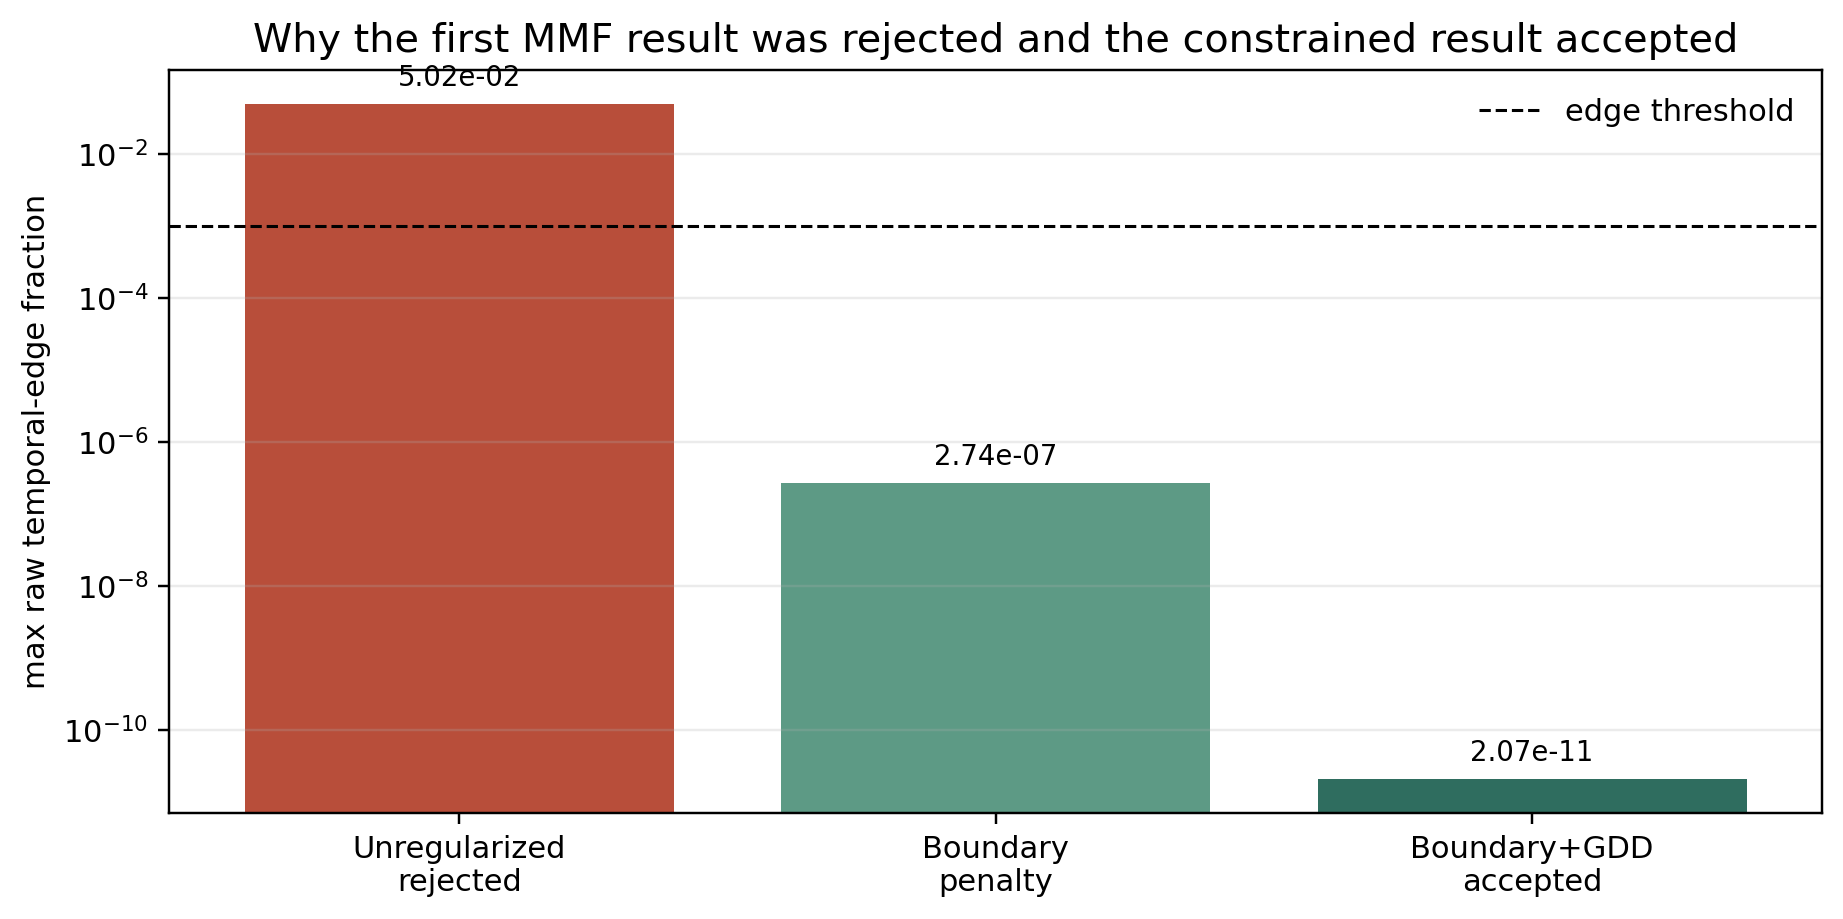
\includegraphics[width=0.80\linewidth]{figures/mmf_edge_trust.png}
\caption{The unregularized solution is rejected because its raw edge fraction
is too high. Boundary and GDD regularization recover strong suppression while
driving the raw edge fraction far below the trust threshold.}
\end{figure}

\subsection*{TL;DR for the Trust Gate}

If a pulse reaches the edge of the simulated time window, the FFT can wrap it
around as if time were periodic. A result can then look good for the wrong
reason. The accepted MMF result is important because it survives the raw-edge
check, not just because it has a low Raman number.

\section{Implementation Surface}

\subsection*{Provenance and Reproducibility Check}

The accepted numbers in this note come from the dedicated MMF window-validation
driver, not from a presentation-only plotting script. The run wrote the
standard image set, the mode-resolved spectra, and the validation summary. It
was then visually inspected because the core risk in this lane is numerical
trust, not just whether an optimizer prints a lower objective.

The accepted run is intentionally modest: \(N_t=4096\), \(96\,\mathrm{ps}\),
six scalar modes, and four optimizer iterations. Attempts to push the same
case to \(N_t=8192\) were compute-limited and did not produce accepted standard
artifacts. This is why the claim is a qualified simulation finding rather than
a paper-grade MMF generalization.

\subsection*{Code Path}

\begin{tabularx}{\linewidth}{@{}p{0.34\linewidth}X@{}}
\toprule
\textbf{Component} & \textbf{Role} \\
\midrule
MMF setup & Builds the GRIN-50 preset, mode launch, grid, fiber, and Raman band. \\
Shared-phase optimizer & Computes the MMF forward solve, adjoint solve, summed objective, and shared phase gradient. \\
Window-validation driver & Reruns the threshold MMF case with larger windows and regularizers, then writes the validation summary. \\
Cost helpers & Provide summed, fundamental-mode, and worst-mode Raman fractions. \\
Standard-image helper & Saves phase profile, phase diagnostic, optimized heat map, and no-shaping heat map. \\
Front-layer config & Supports planning and dry-run validation only; real MMF propagation remains burst/heavy-compute work. \\
\bottomrule
\end{tabularx}

\section{Experimental Ladder}

\begin{figure}[H]
\centering
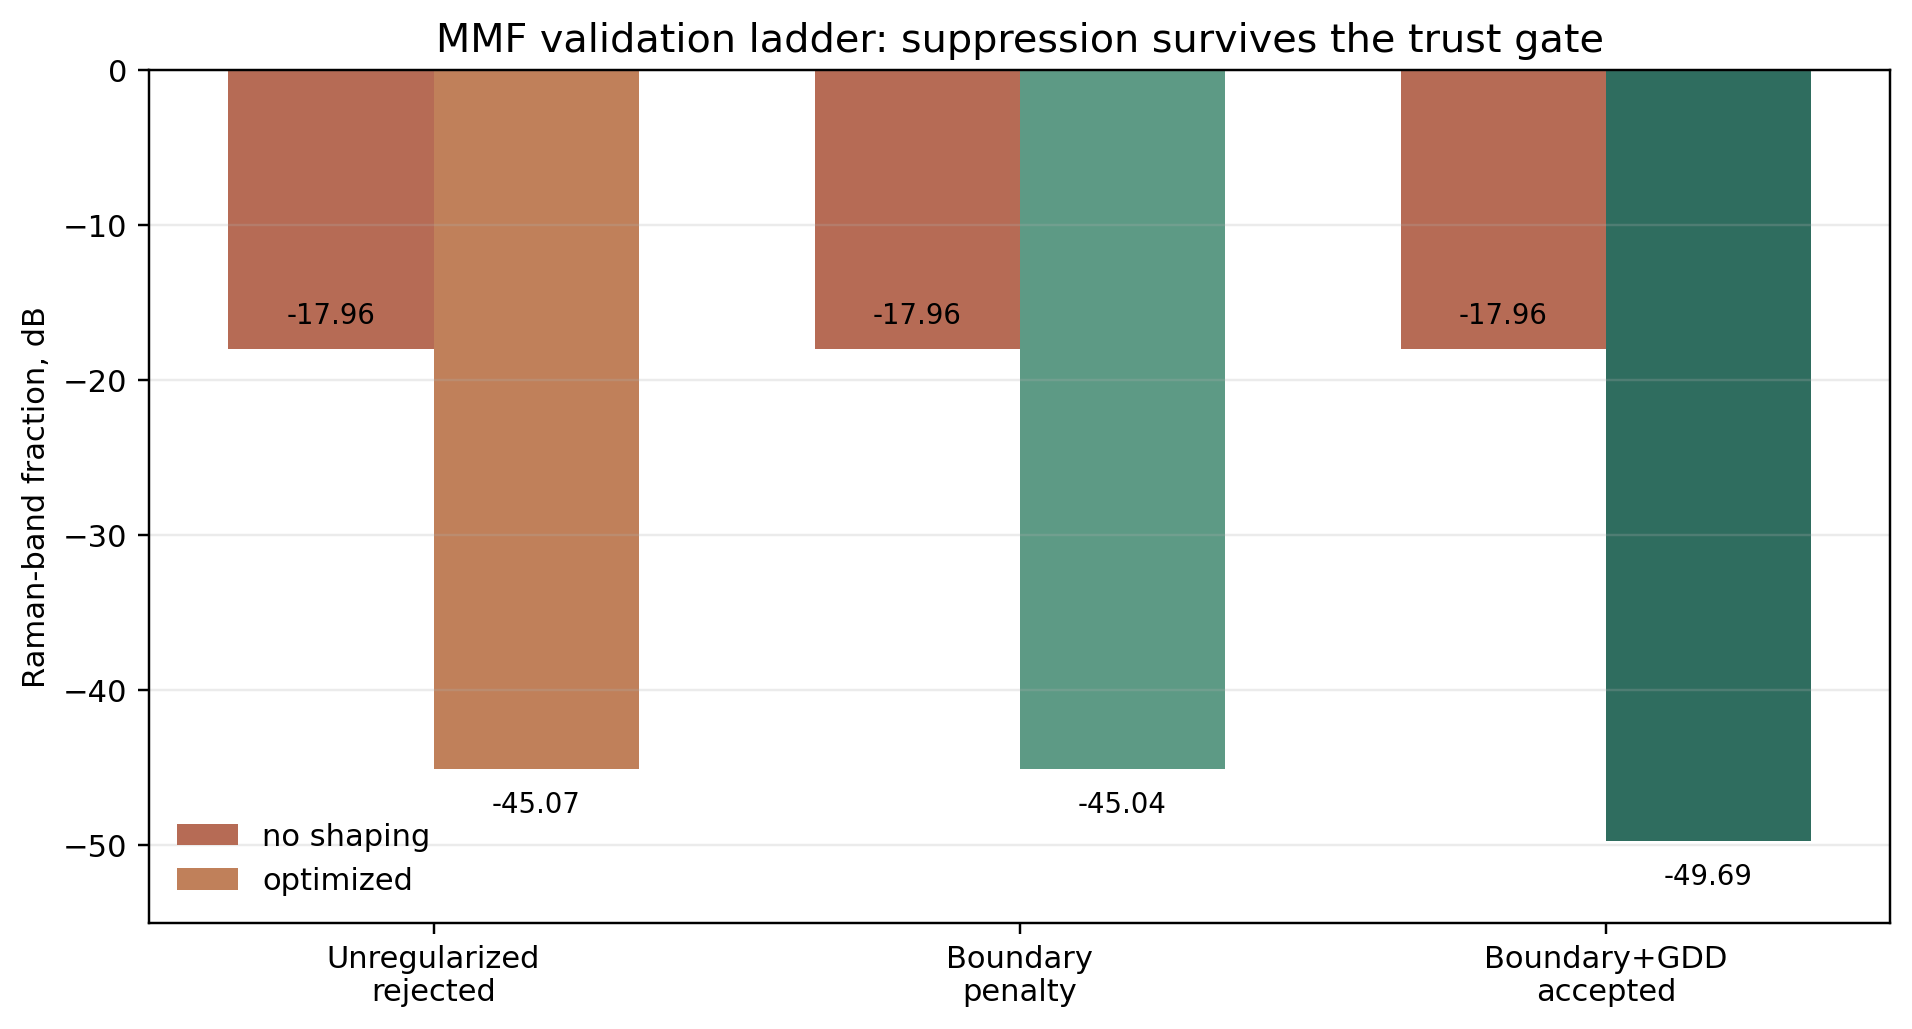
\includegraphics[width=0.88\linewidth]{figures/mmf_validation_ladder.png}
\caption{MMF validation ladder. The final accepted result is not just the
deepest-looking run; it is the deepest run that also passes the raw temporal
edge diagnostics among the tested candidates.}
\end{figure}

\begin{table}[H]
\centering
\small
\begin{tabular}{@{}lrrrr@{}}
\toprule
\textbf{Case} & \textbf{Objective dB} & \textbf{Improvement} & \textbf{Max edge} & \textbf{Verdict} \\
\midrule
Unregularized & \(-45.07\) & \(27.12\,\mathrm{dB}\) & \(5.02\times10^{-2}\) & reject \\
Boundary penalty & \(-45.04\) & \(27.09\,\mathrm{dB}\) & \(2.74\times10^{-7}\) & pass \\
Boundary+GDD & \(-49.69\) & \(31.73\,\mathrm{dB}\) & \(2.07\times10^{-11}\) & accepted \\
\bottomrule
\end{tabular}
\caption{All rows use \(L=2\,\mathrm{m}\), \(P=0.20\,\mathrm{W}\),
\(N_t=4096\), and \(96\,\mathrm{ps}\). The unregularized row is scientifically
useful because it explains what had to be fixed, but it is not accepted as a
valid result.}
\end{table}

\section{Representative Result Pages}

\begin{figure}[p]
\centering
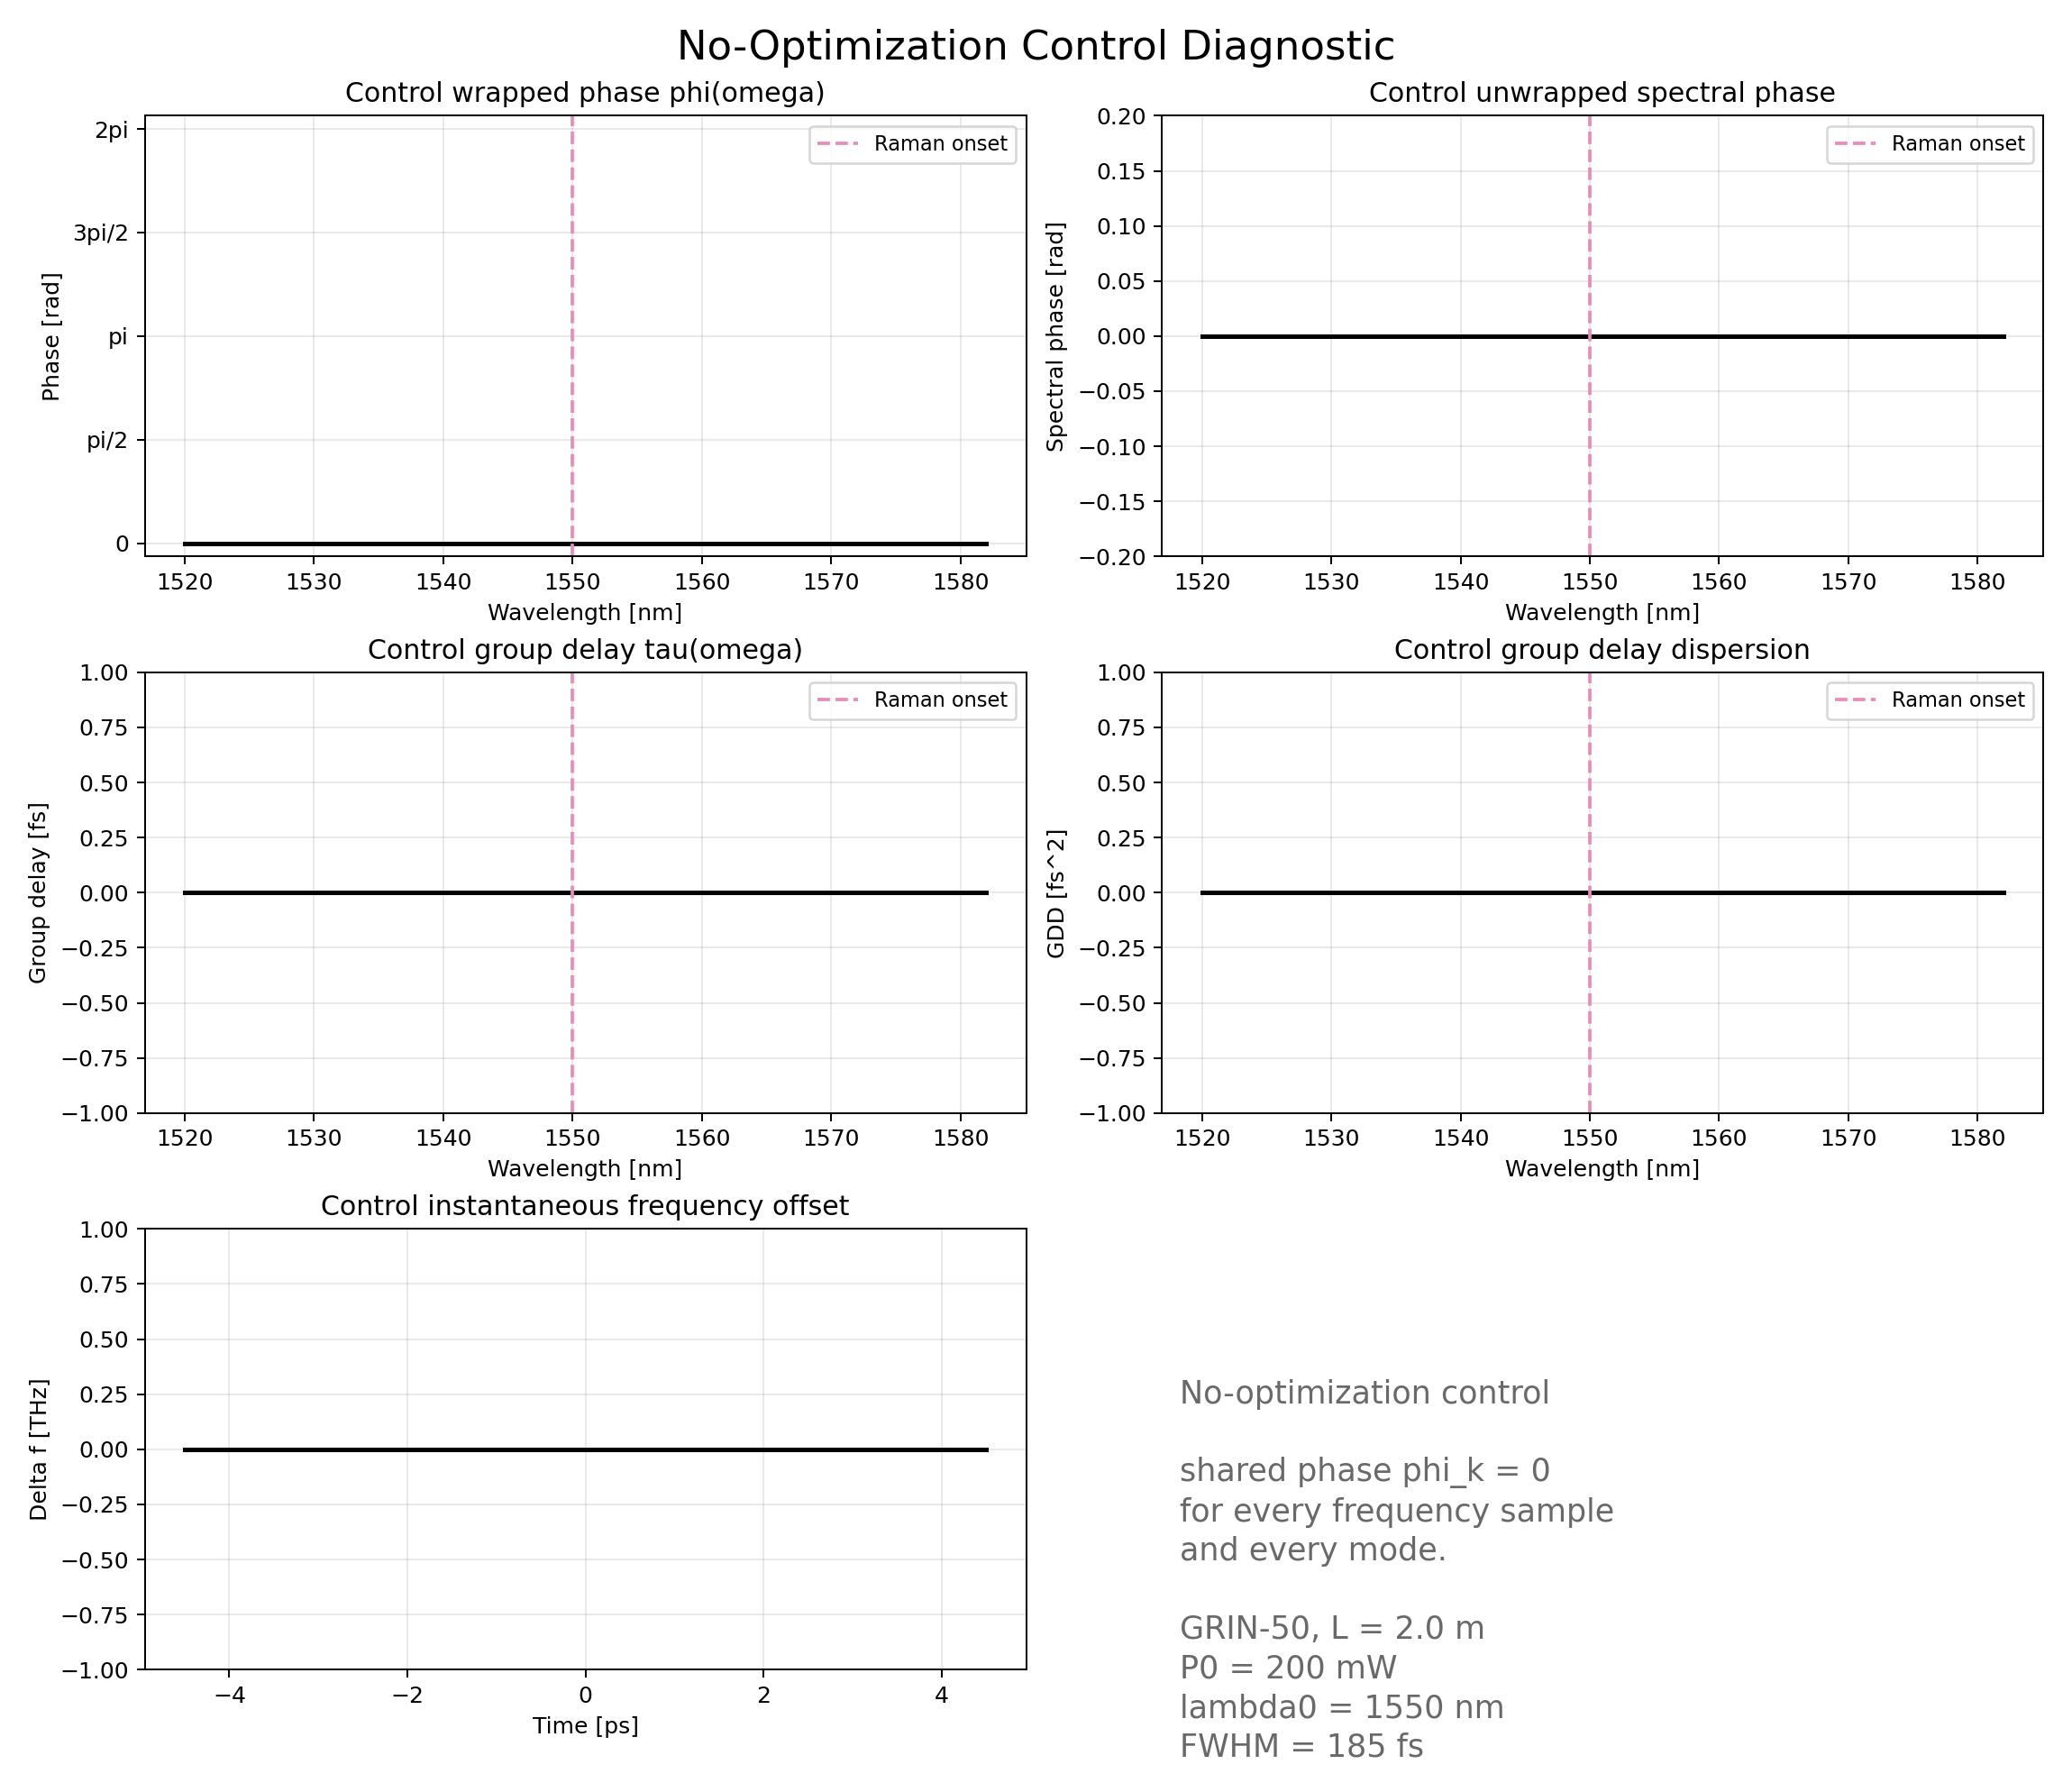
\includegraphics[height=0.52\textheight,keepaspectratio]{figures/mmf_control_phase_diagnostic.png}

\vspace{0.5em}
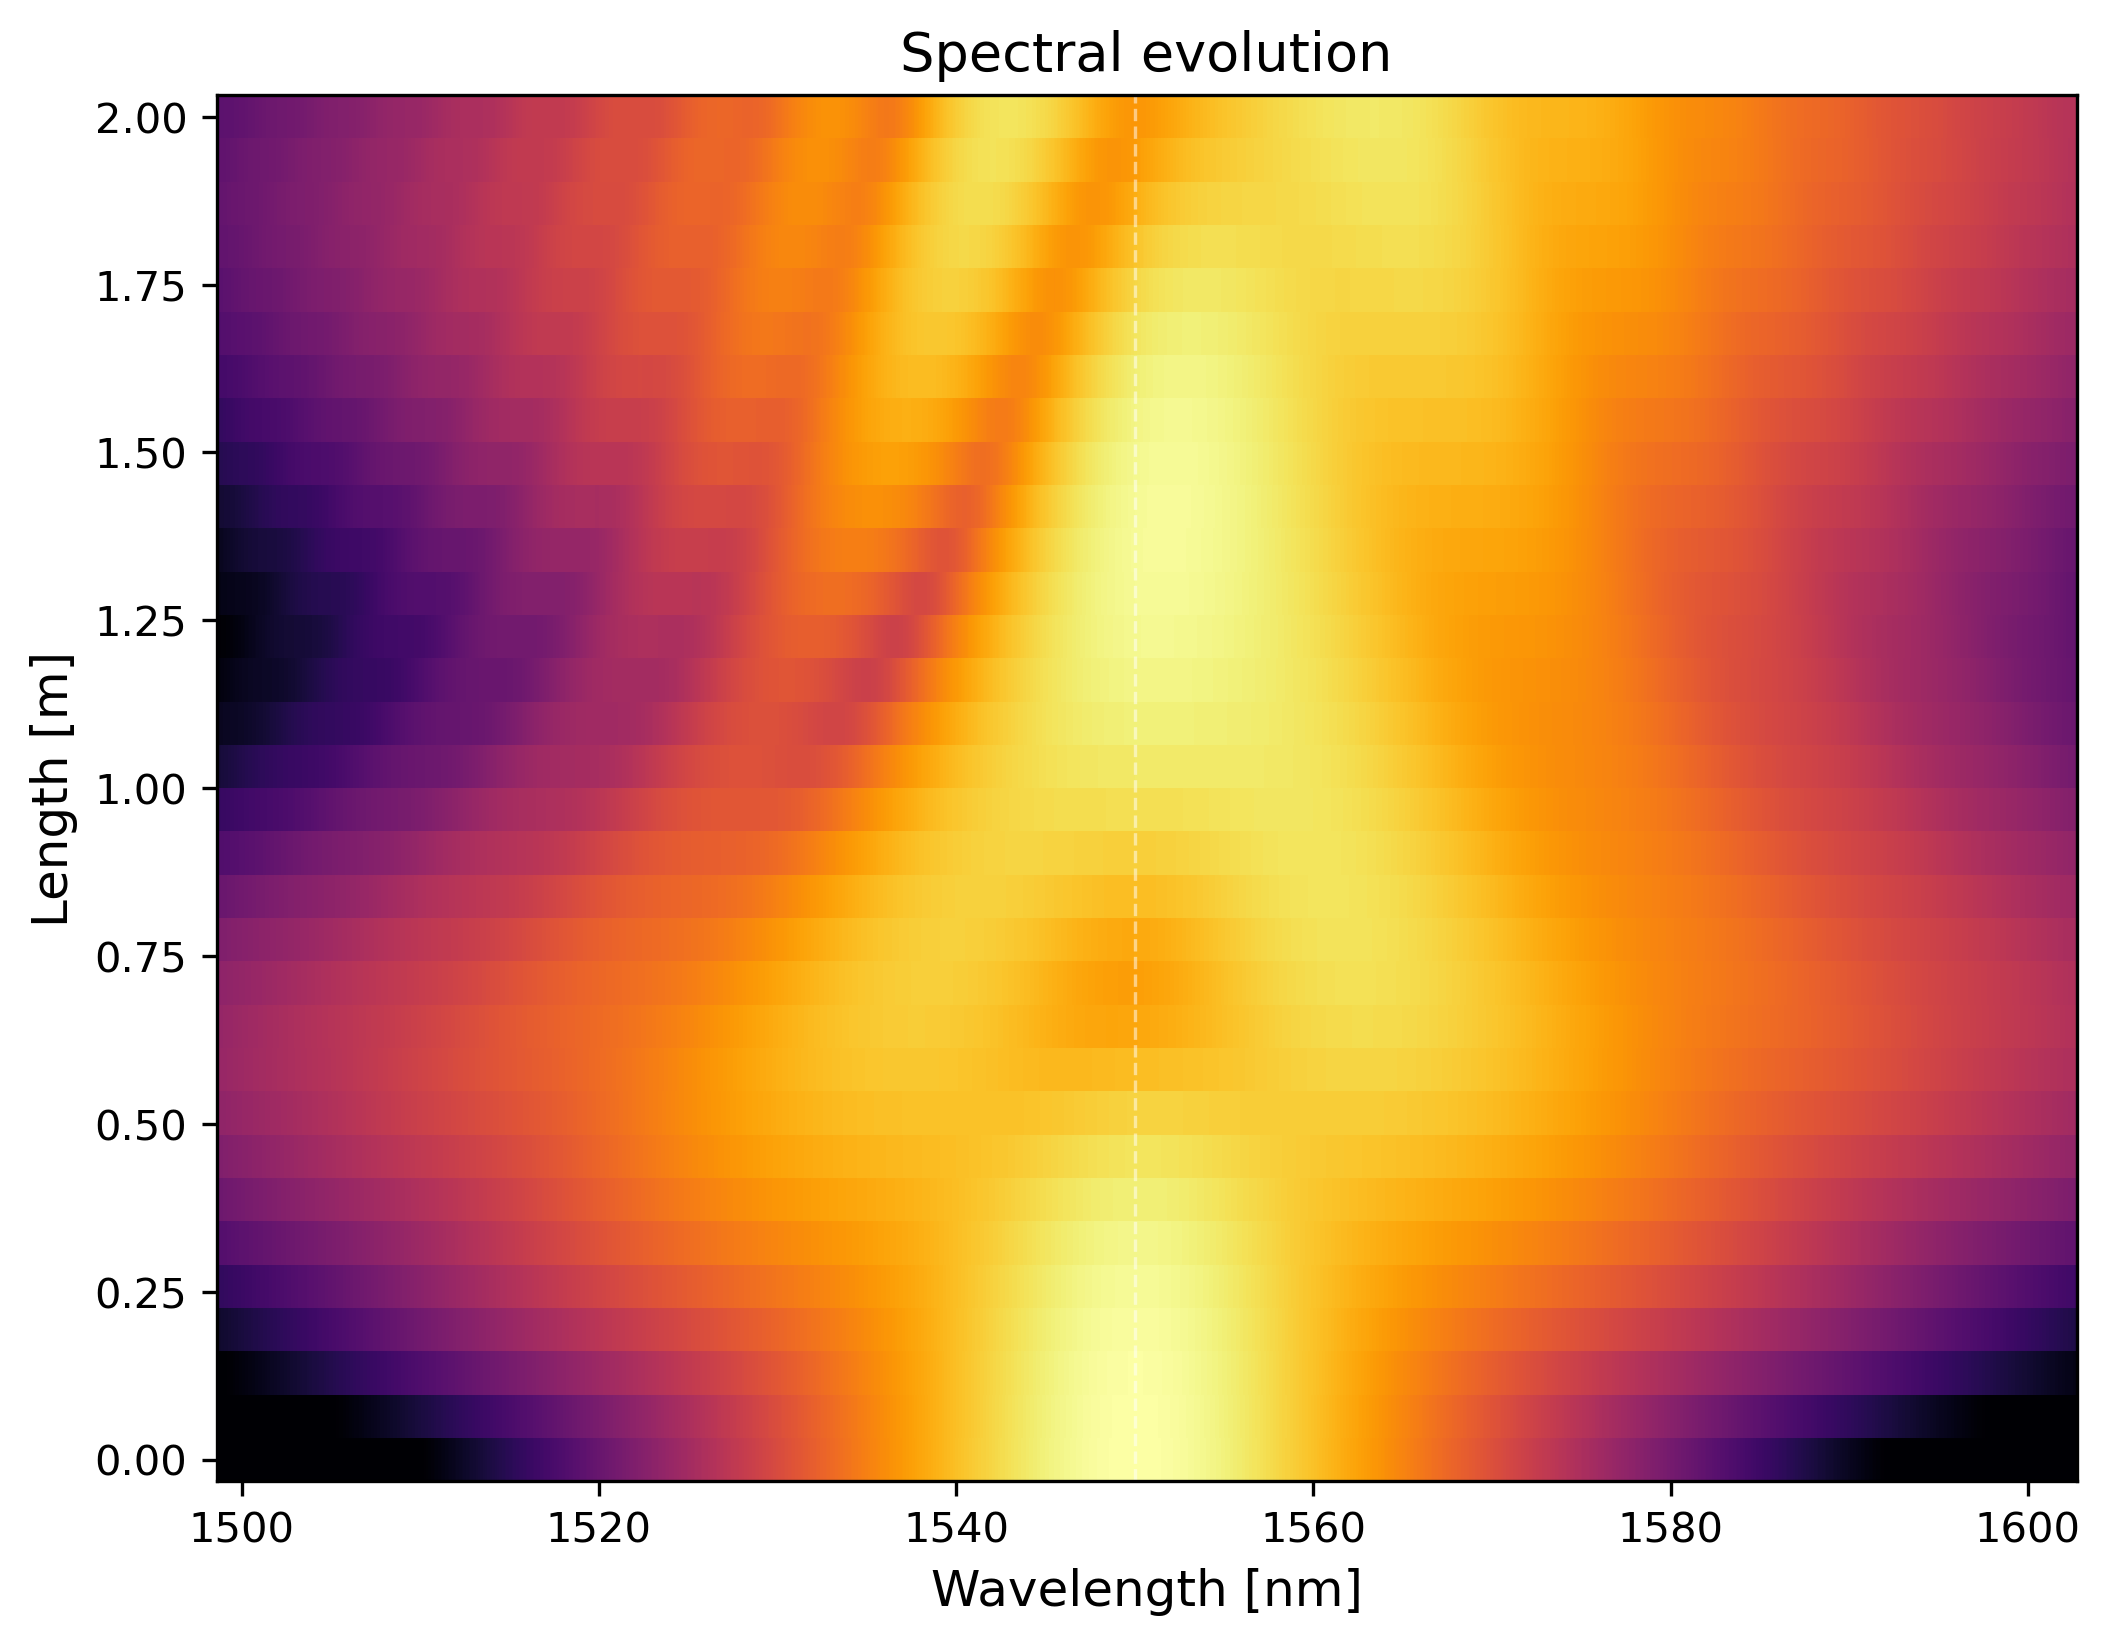
\includegraphics[height=0.34\textheight,keepaspectratio]{figures/mmf_control_evolution.png}
\caption{No-optimization control for the accepted MMF operating point. The top
panel records the flat shared phase \(\phi_k=0\); the bottom panel is the
actual no-shaping spectral-evolution heat map used as the control reference.}
\end{figure}

\begin{figure}[p]
\centering
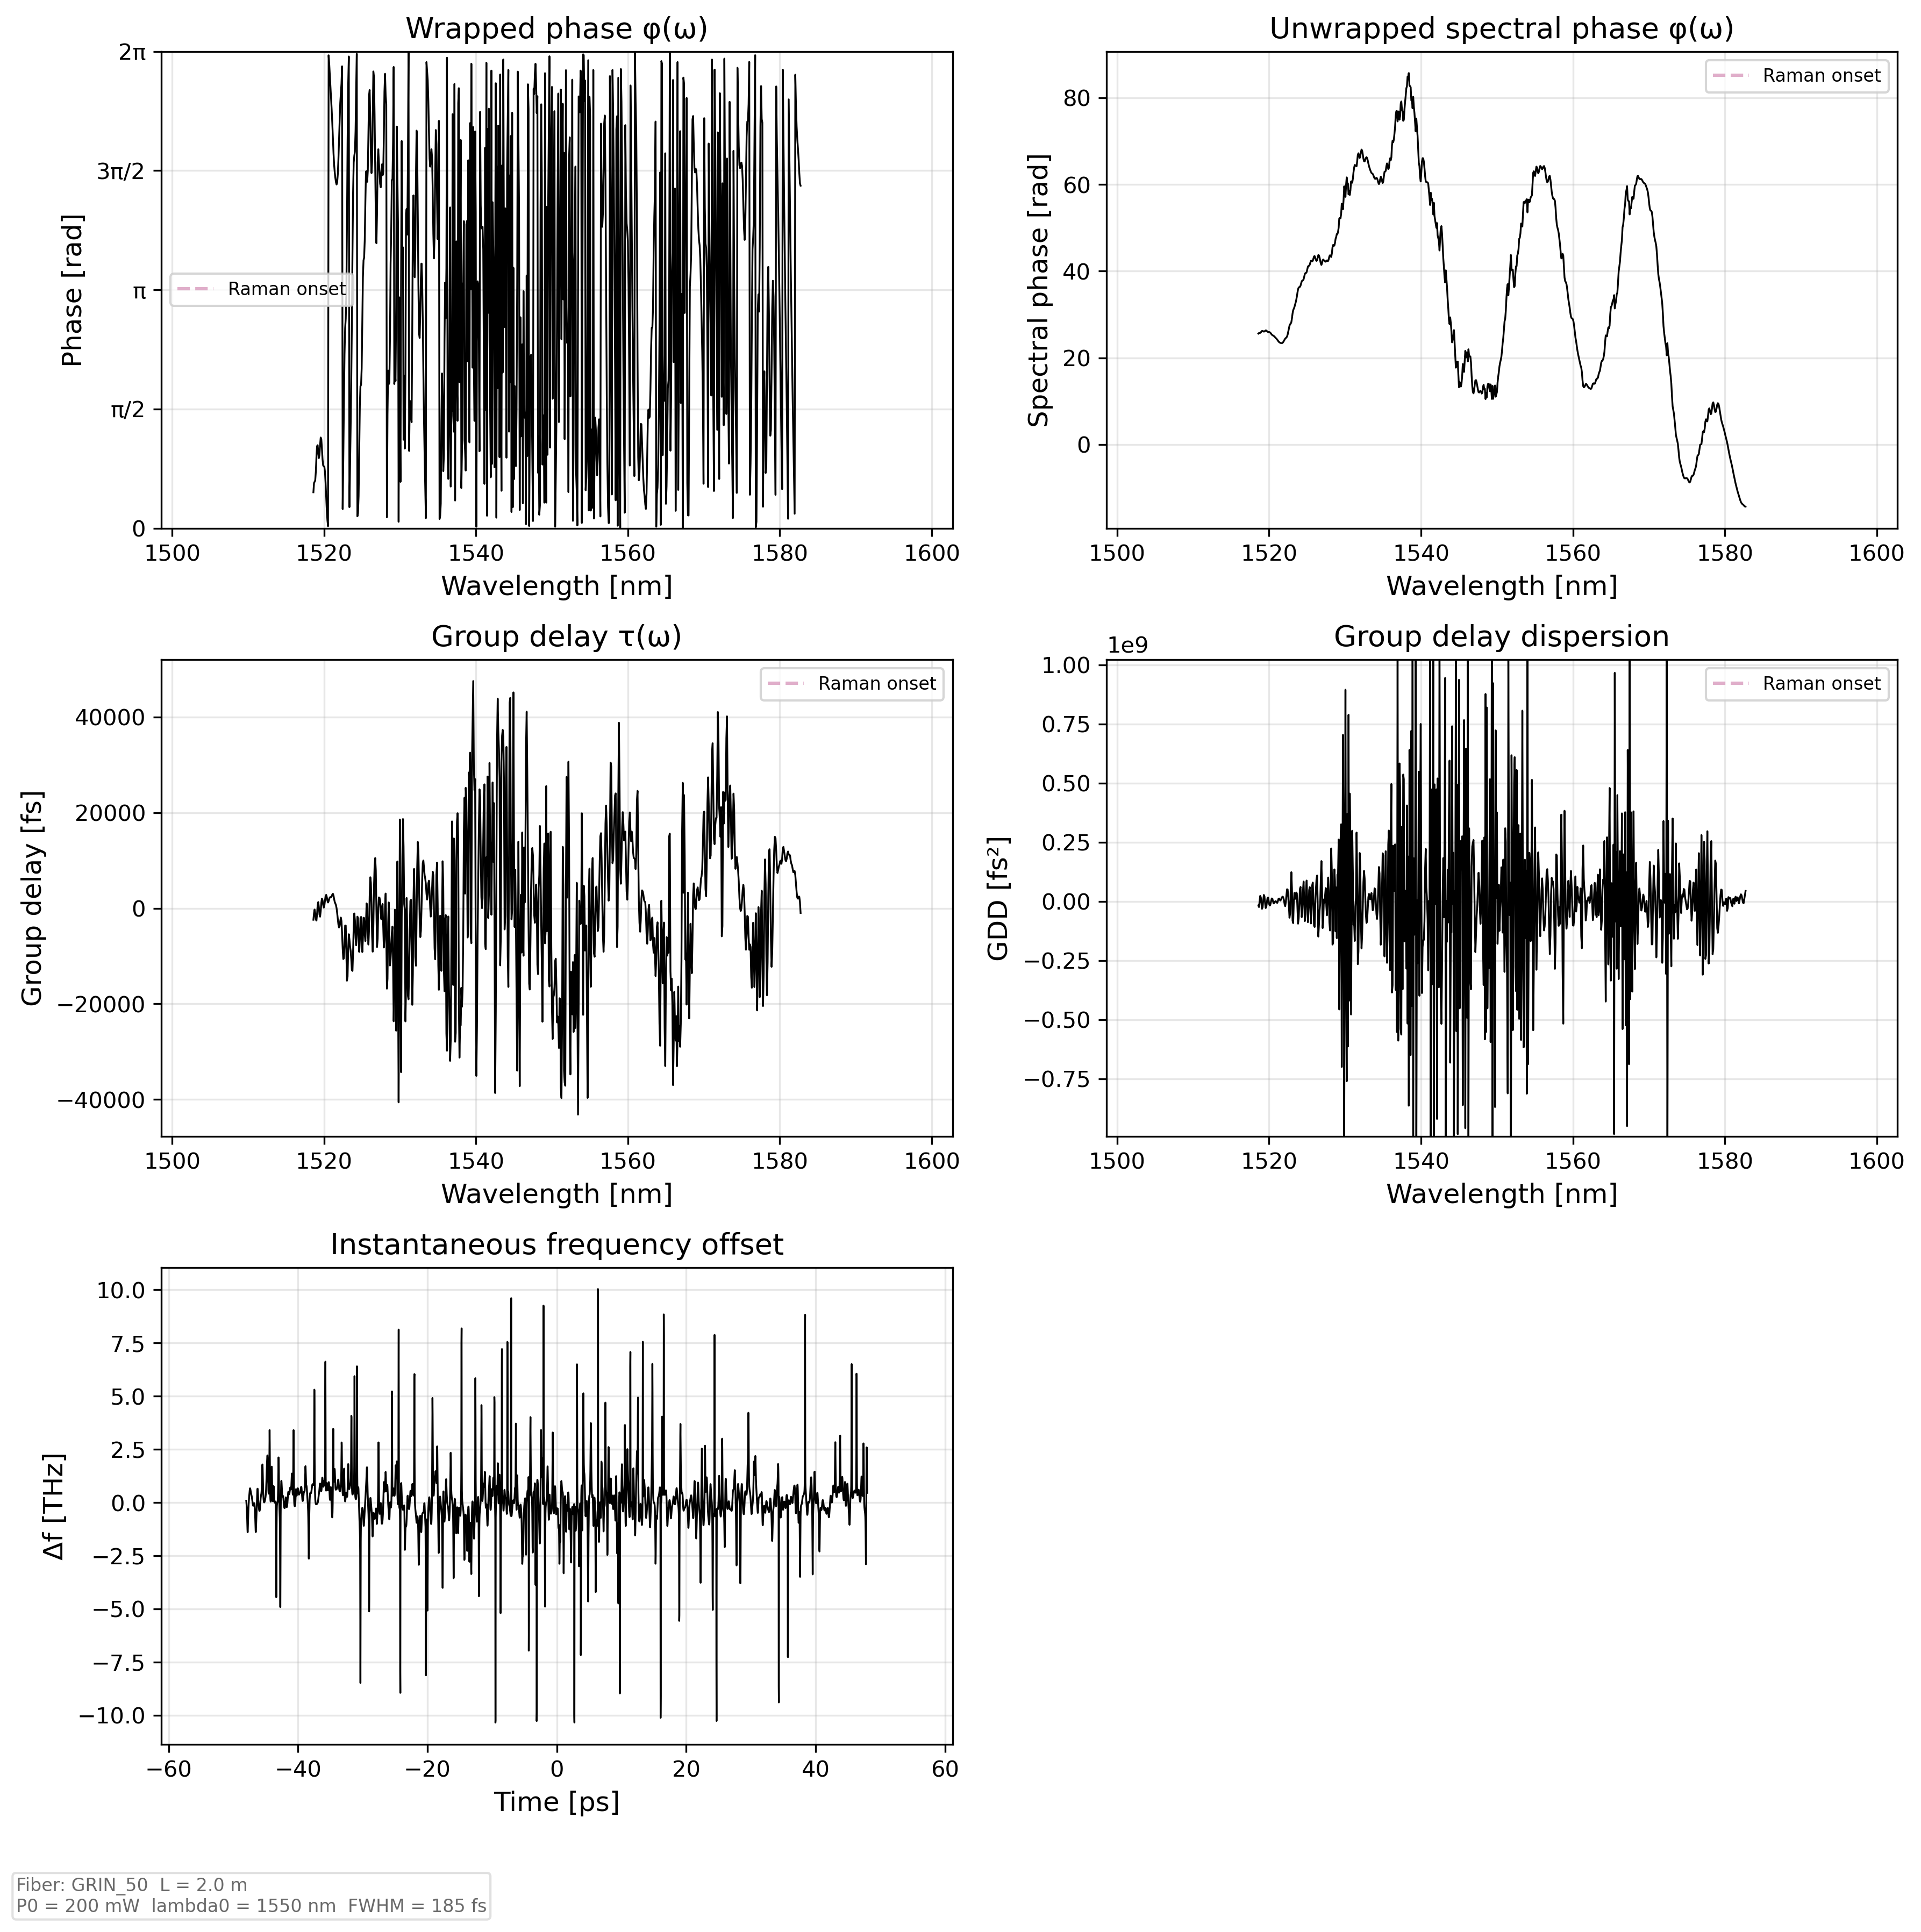
\includegraphics[height=0.52\textheight,keepaspectratio]{figures/mmf_rejected_unregularized_phase_diagnostic.png}

\vspace{0.5em}
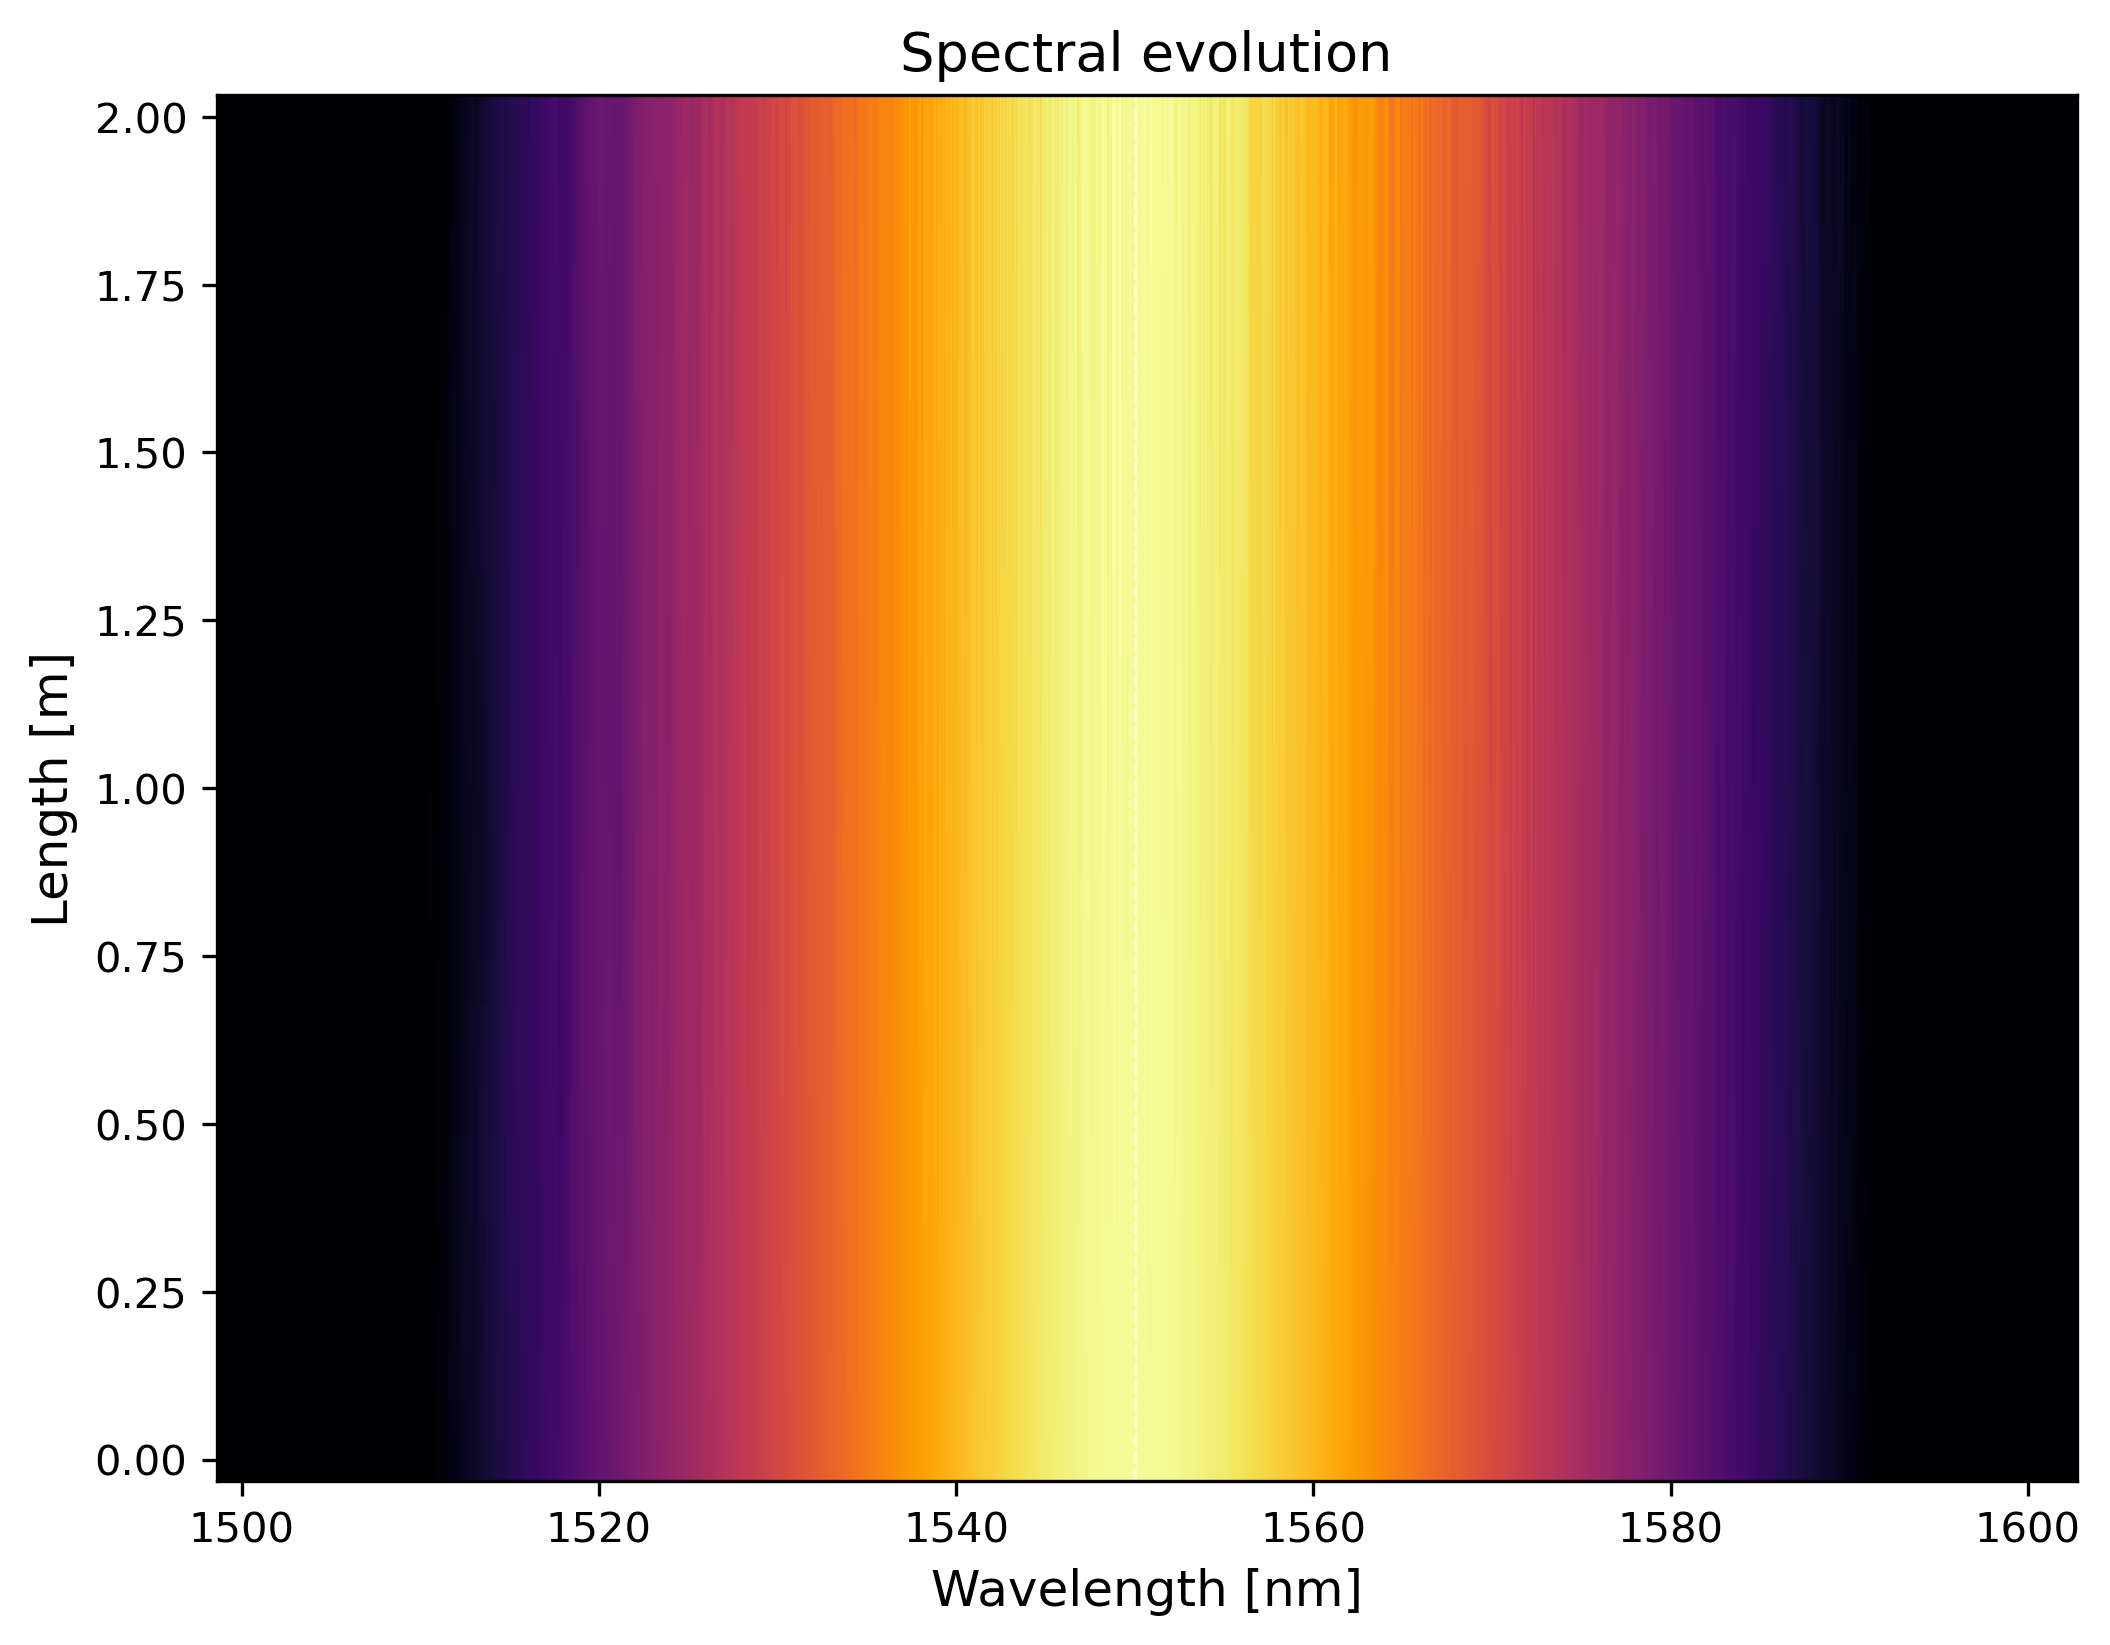
\includegraphics[height=0.34\textheight,keepaspectratio]{figures/mmf_rejected_unregularized_evolution.png}
\caption{The unregularized run visually suppresses Raman output, but it is not
accepted because corrected raw-edge diagnostics show temporal-window
contamination.}
\end{figure}

\begin{figure}[p]
\centering
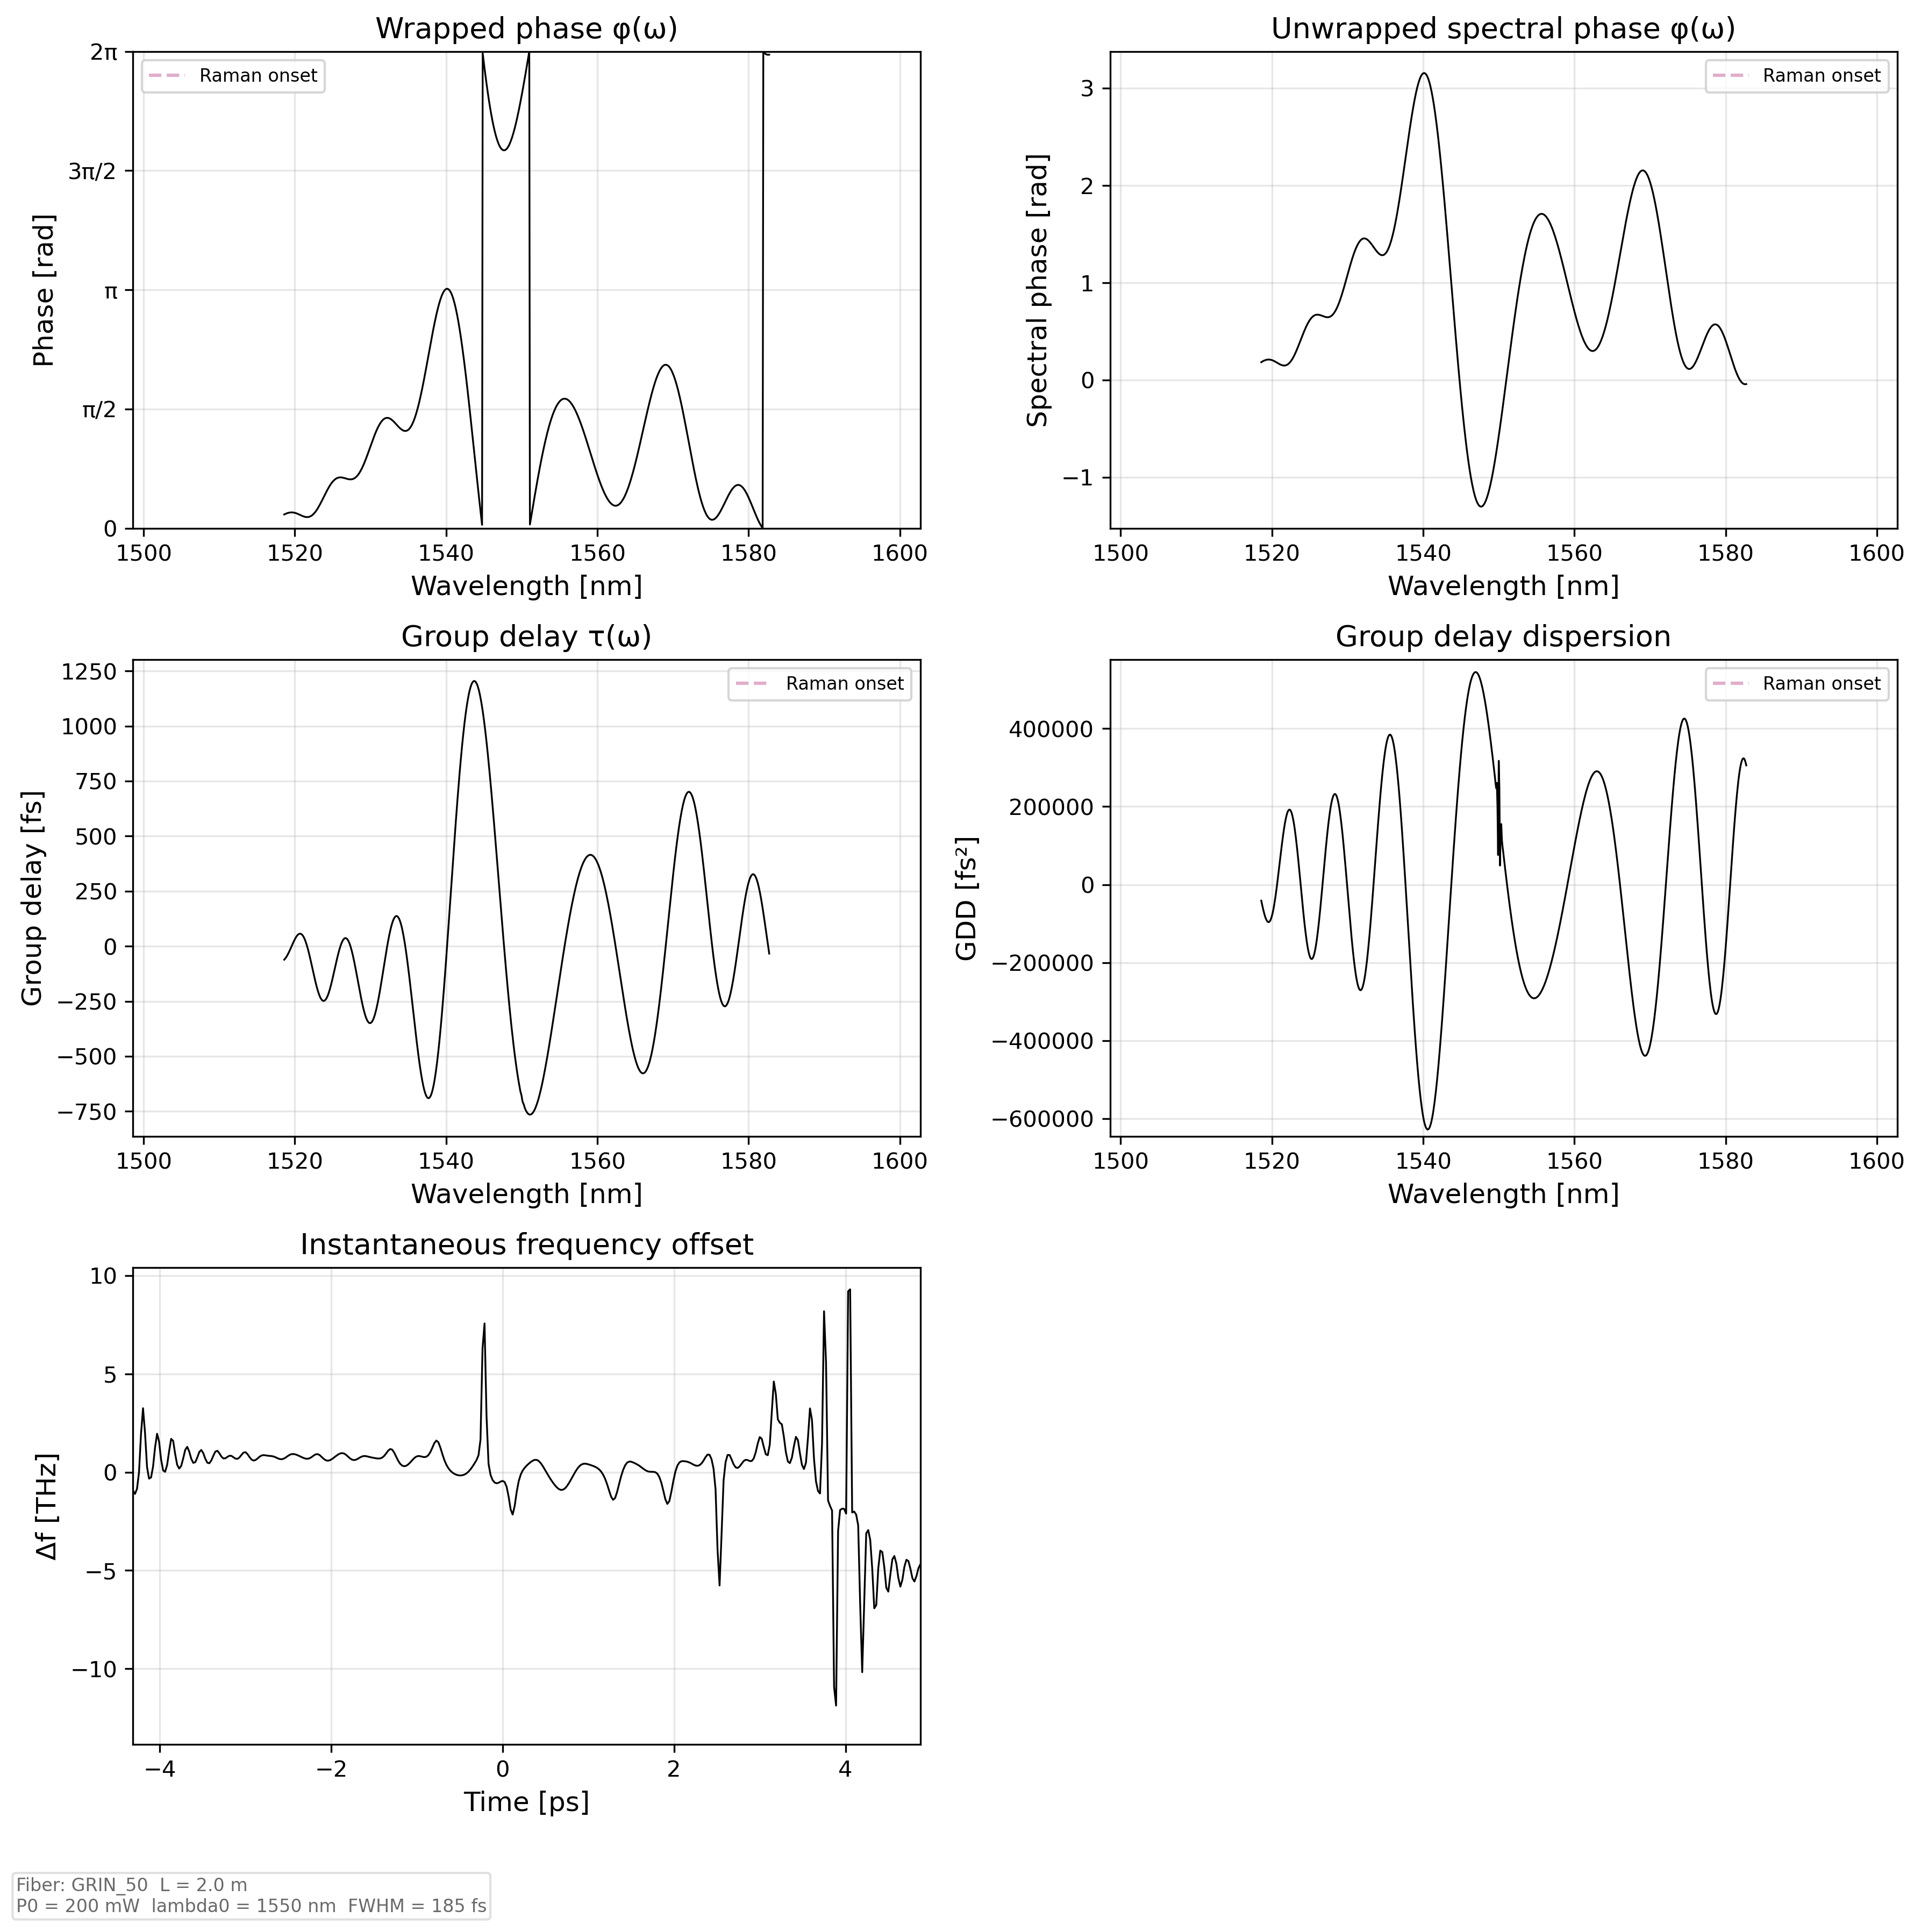
\includegraphics[height=0.52\textheight,keepaspectratio]{figures/mmf_accepted_phase_diagnostic.png}

\vspace{0.5em}
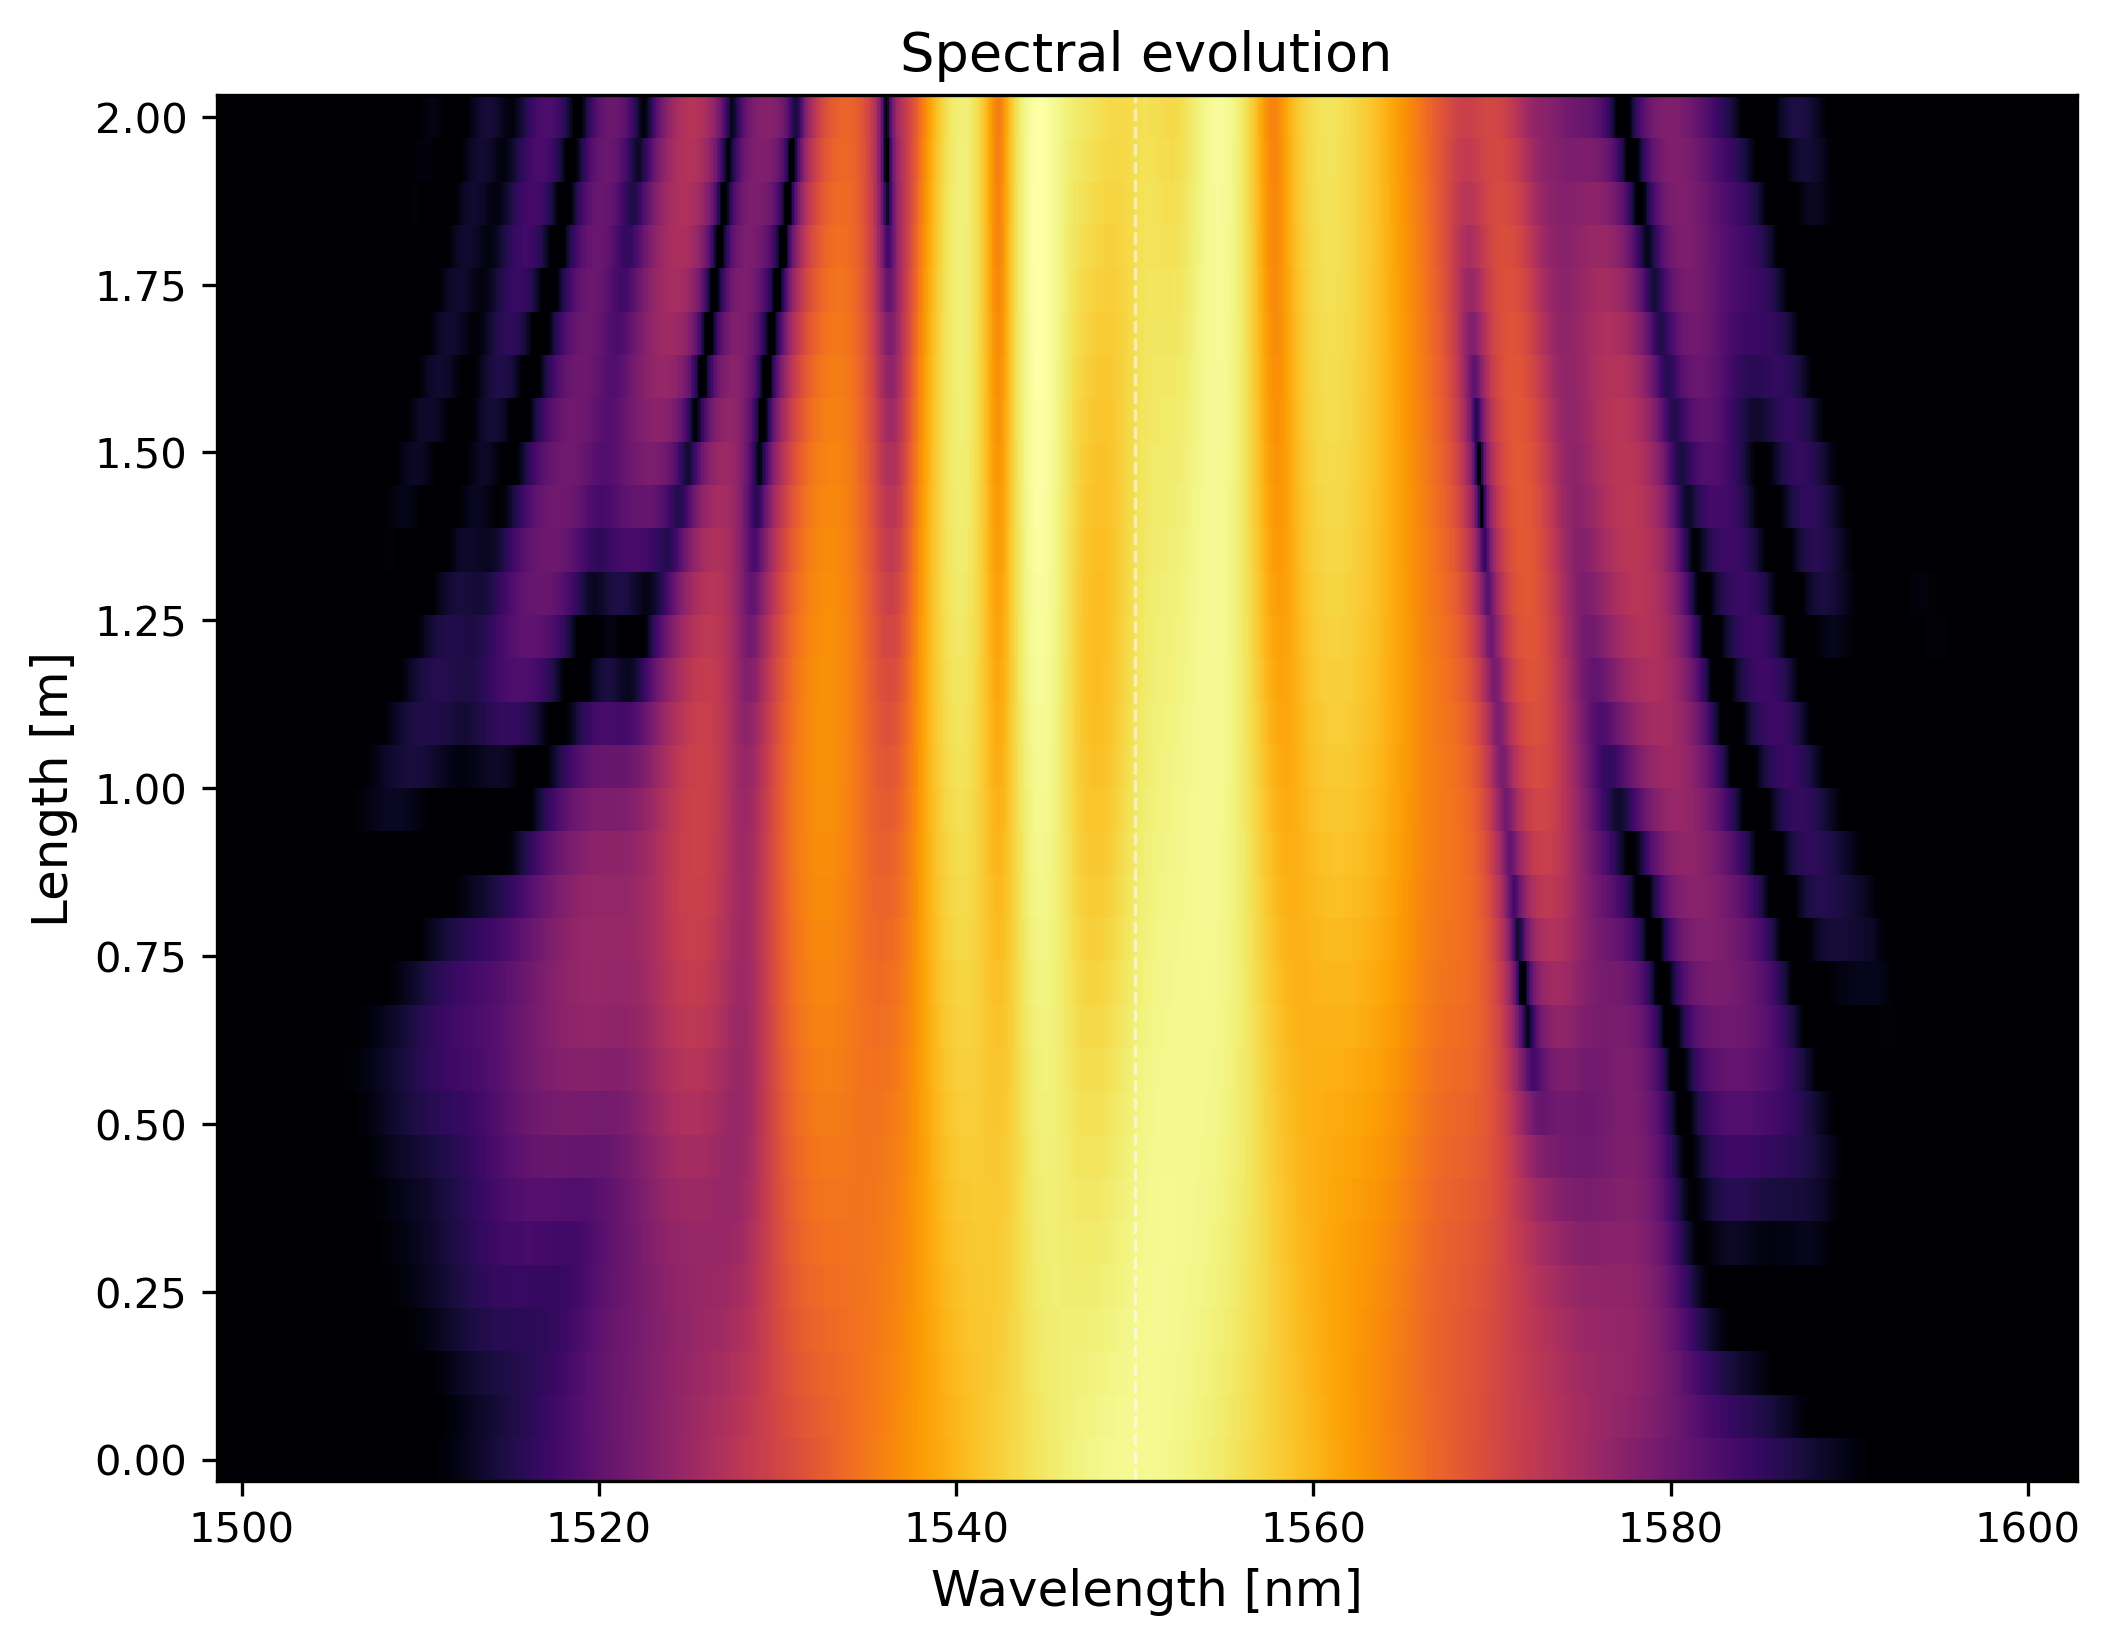
\includegraphics[height=0.34\textheight,keepaspectratio]{figures/mmf_accepted_evolution.png}
\caption{Accepted constrained MMF result: \(-17.96\rightarrow -49.69\,\mathrm{dB}\) under the mode-summed Raman objective, with raw edge fractions near \(2\times10^{-11}\).}
\end{figure}

\begin{figure}[H]
\centering
\begin{minipage}{0.48\linewidth}
\centering
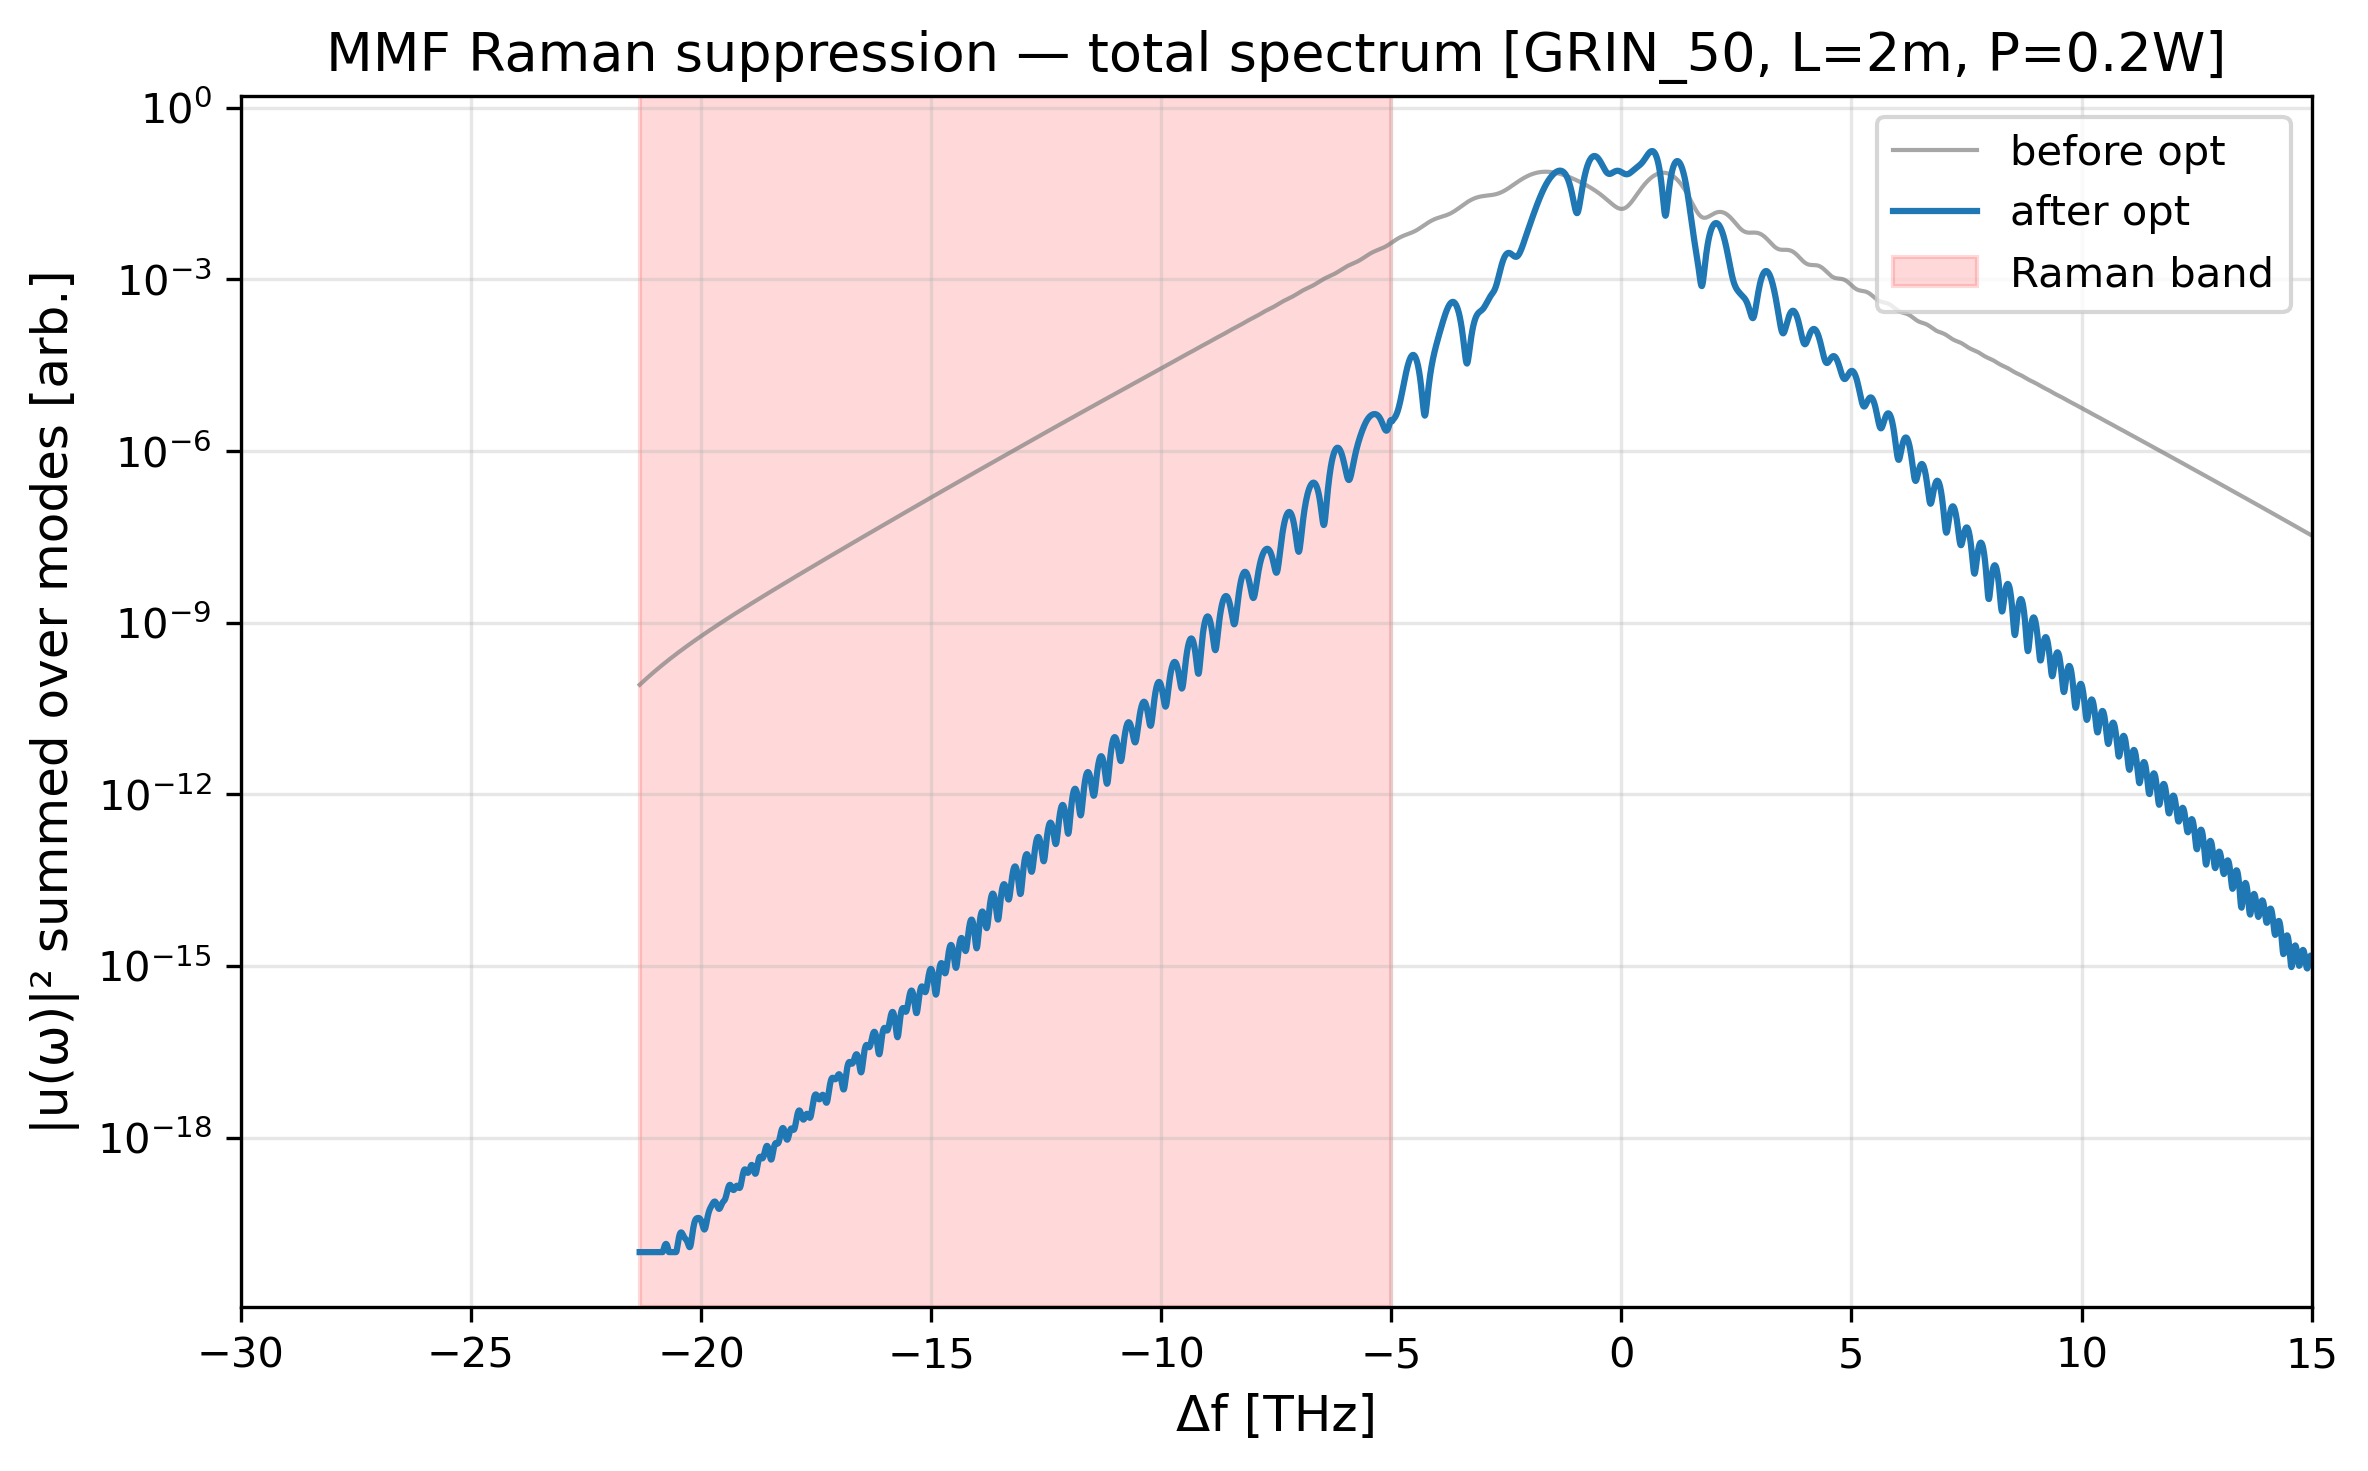
\includegraphics[width=\linewidth]{figures/mmf_accepted_total_spectrum.png}
\caption*{Total spectrum.}
\end{minipage}
\hfill
\begin{minipage}{0.48\linewidth}
\centering
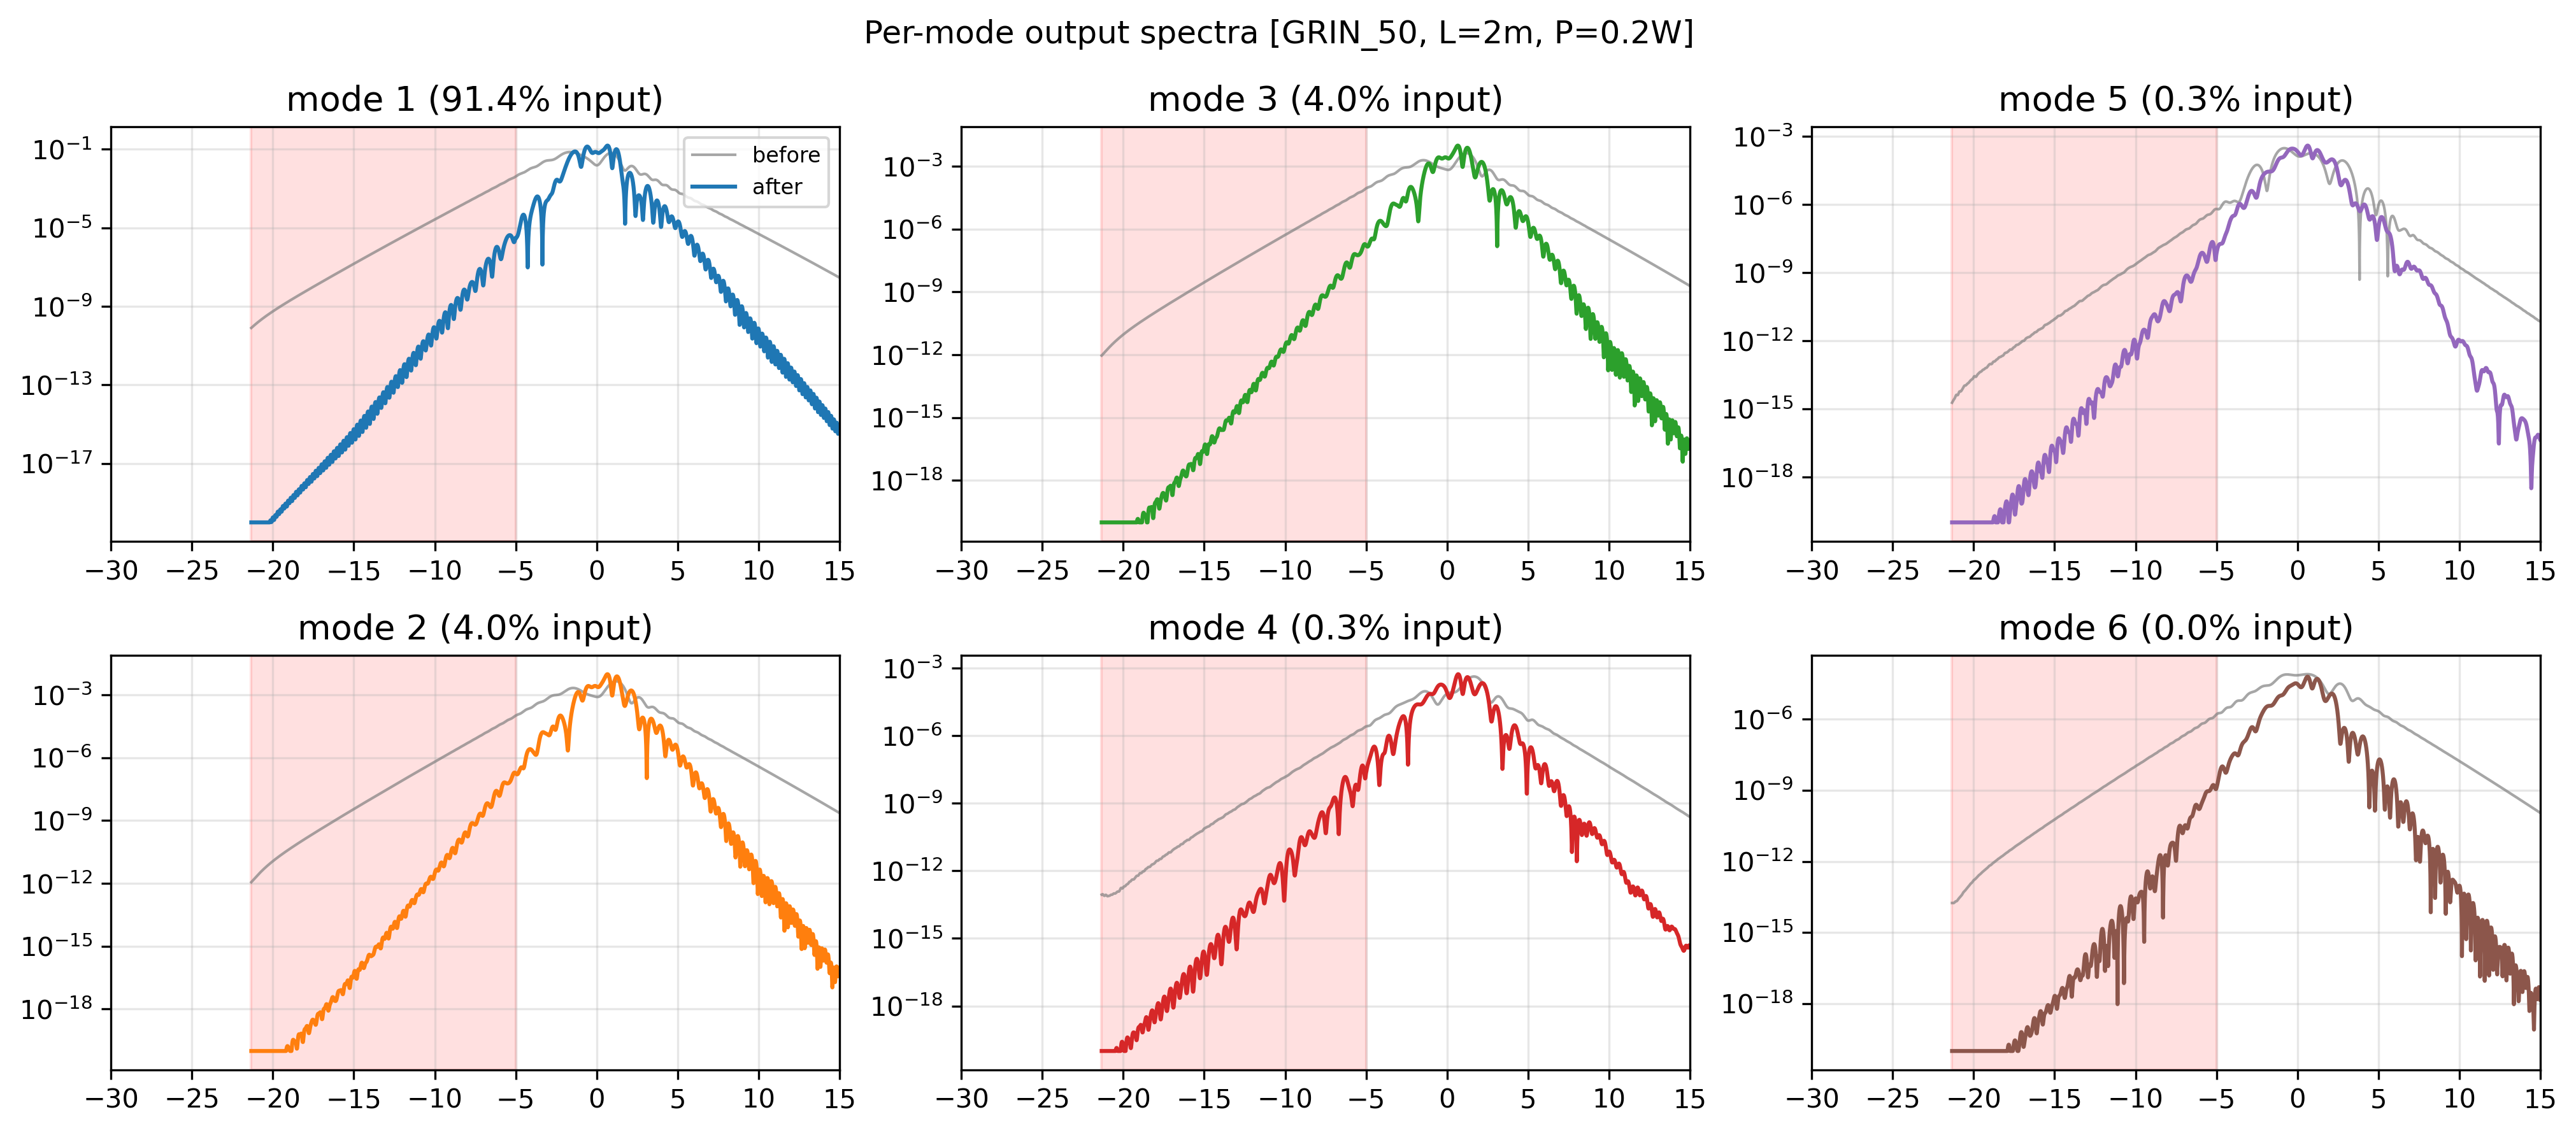
\includegraphics[width=\linewidth]{figures/mmf_accepted_per_mode_spectrum.png}
\caption*{Per-mode spectrum.}
\end{minipage}
\caption{Mode-resolved inspection matters. The accepted run is not only a
summed-detector accounting win; the launched modes also show suppression.}
\end{figure}

\begin{figure}[H]
\centering
\begin{minipage}{0.48\linewidth}
\centering
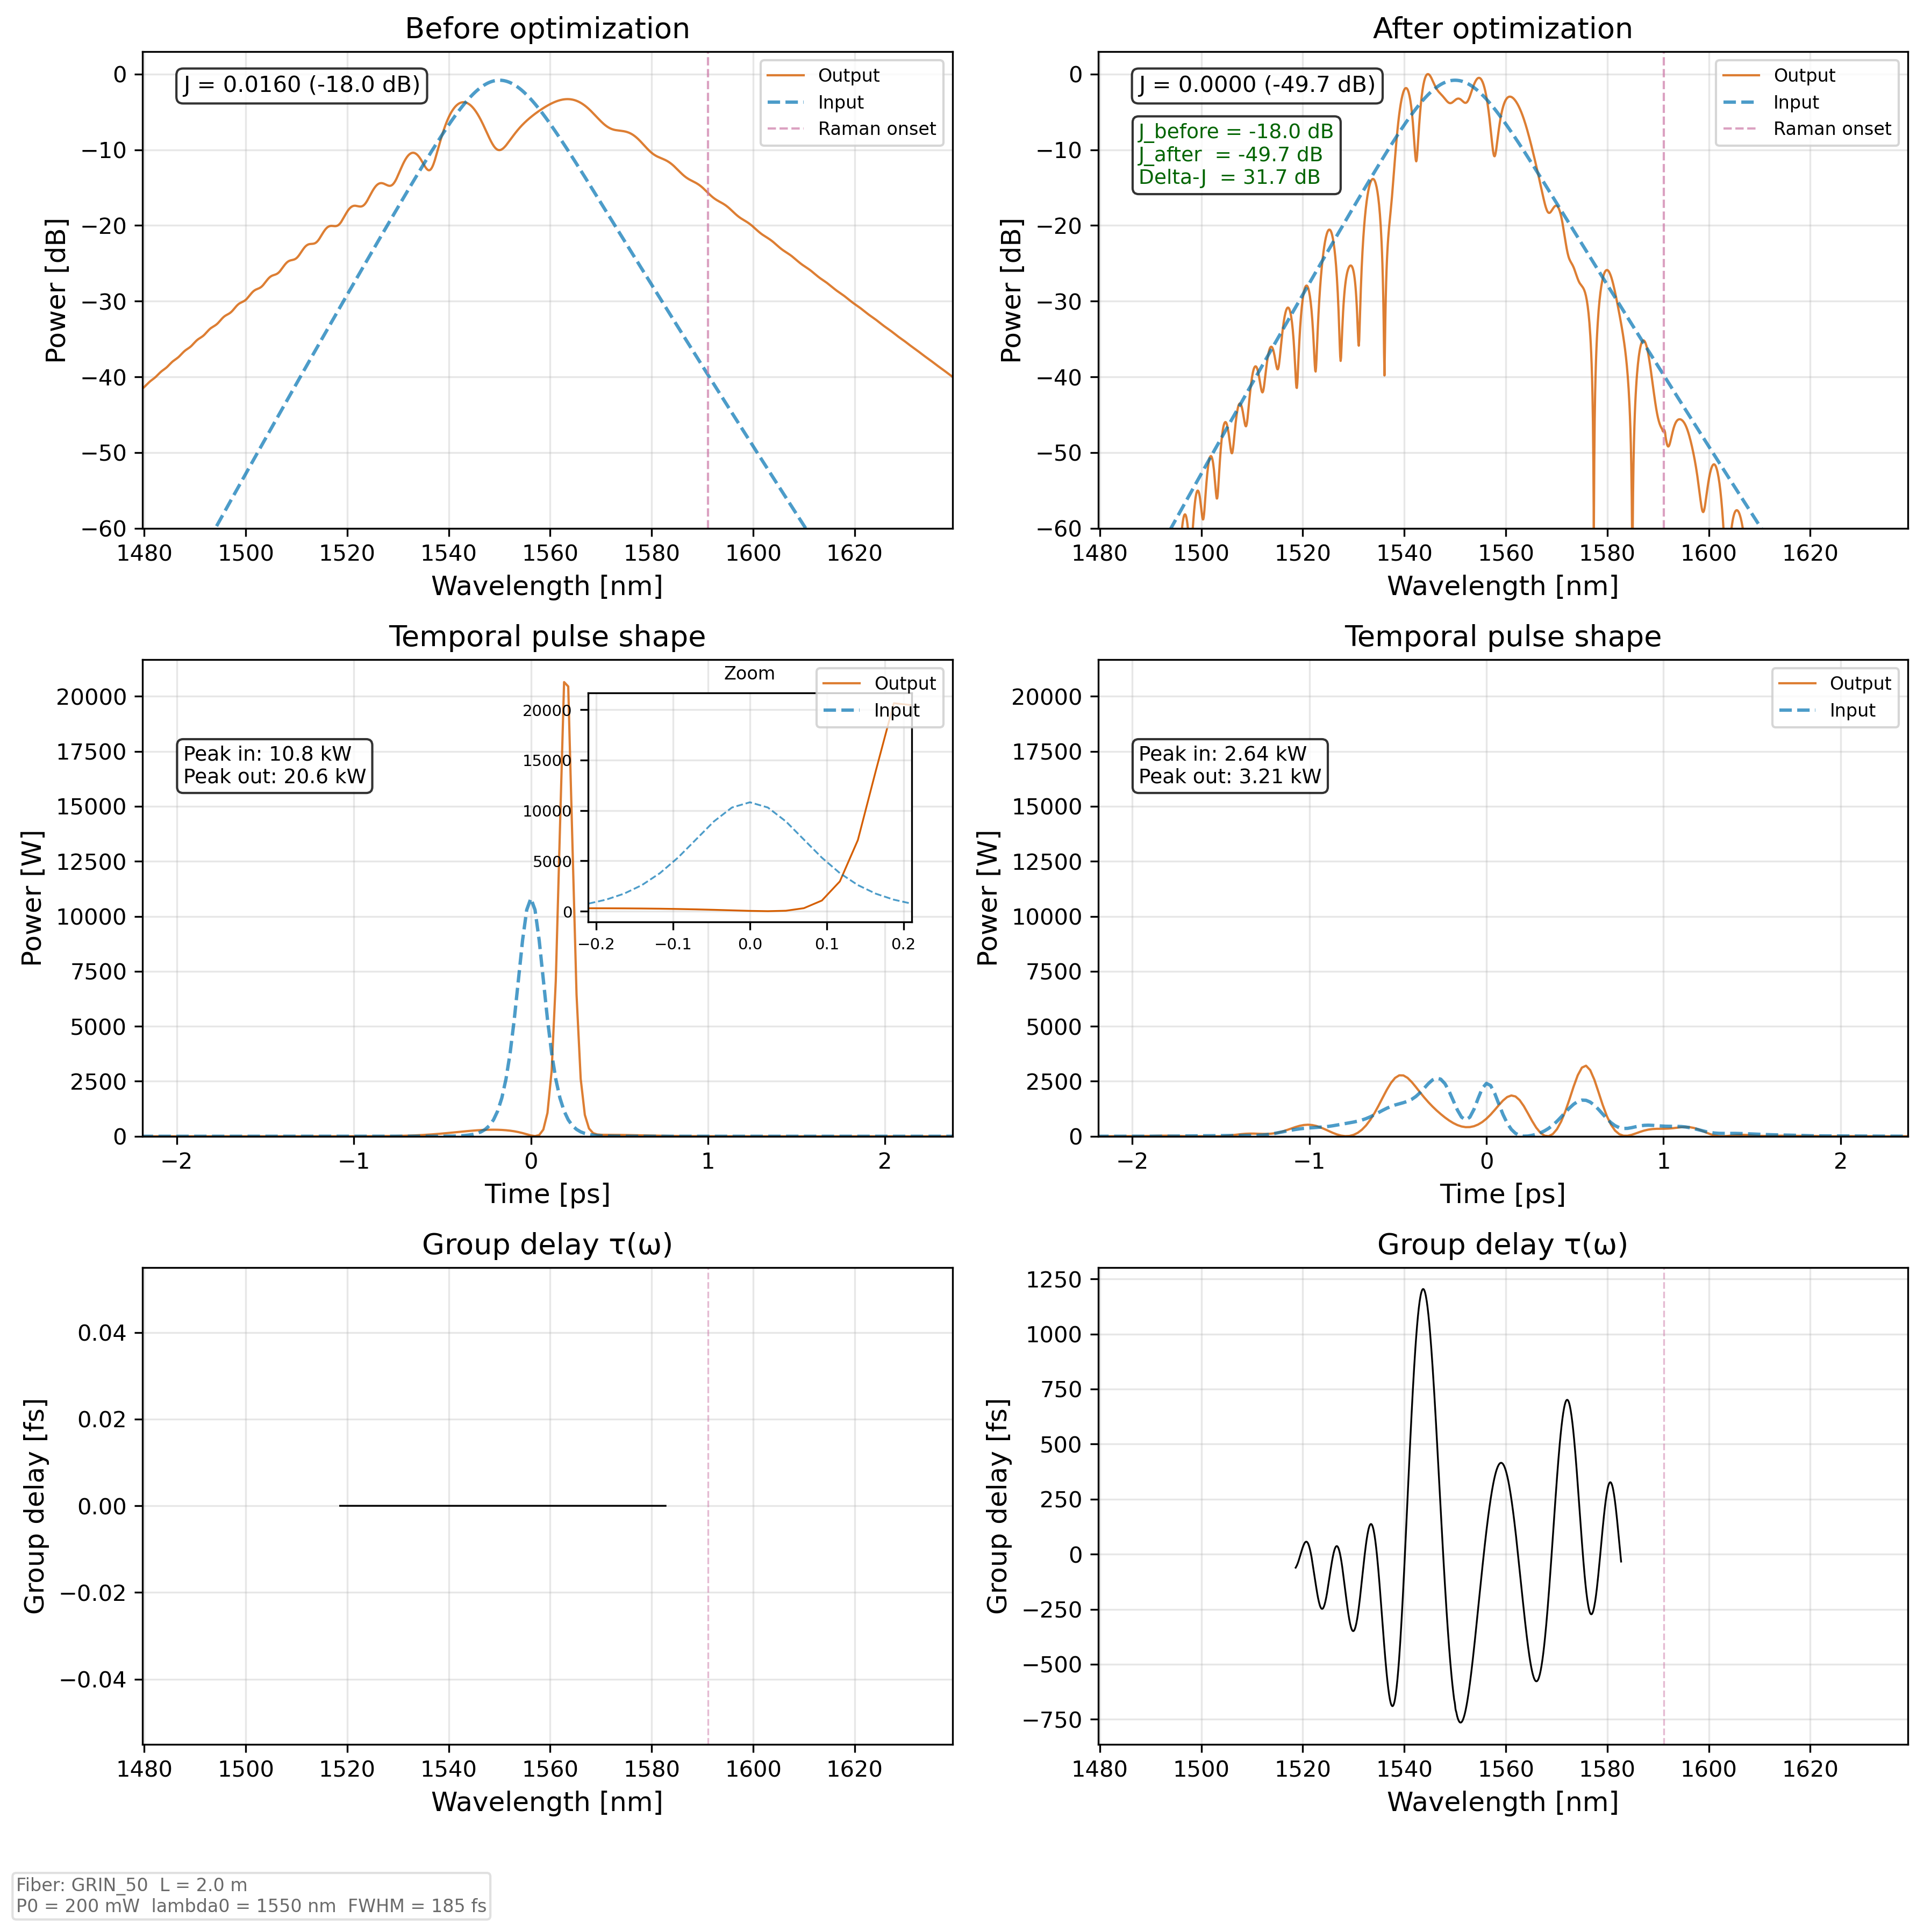
\includegraphics[width=\linewidth]{figures/mmf_accepted_phase_profile.png}
\caption*{Accepted phase profile.}
\end{minipage}
\hfill
\begin{minipage}{0.48\linewidth}
\centering
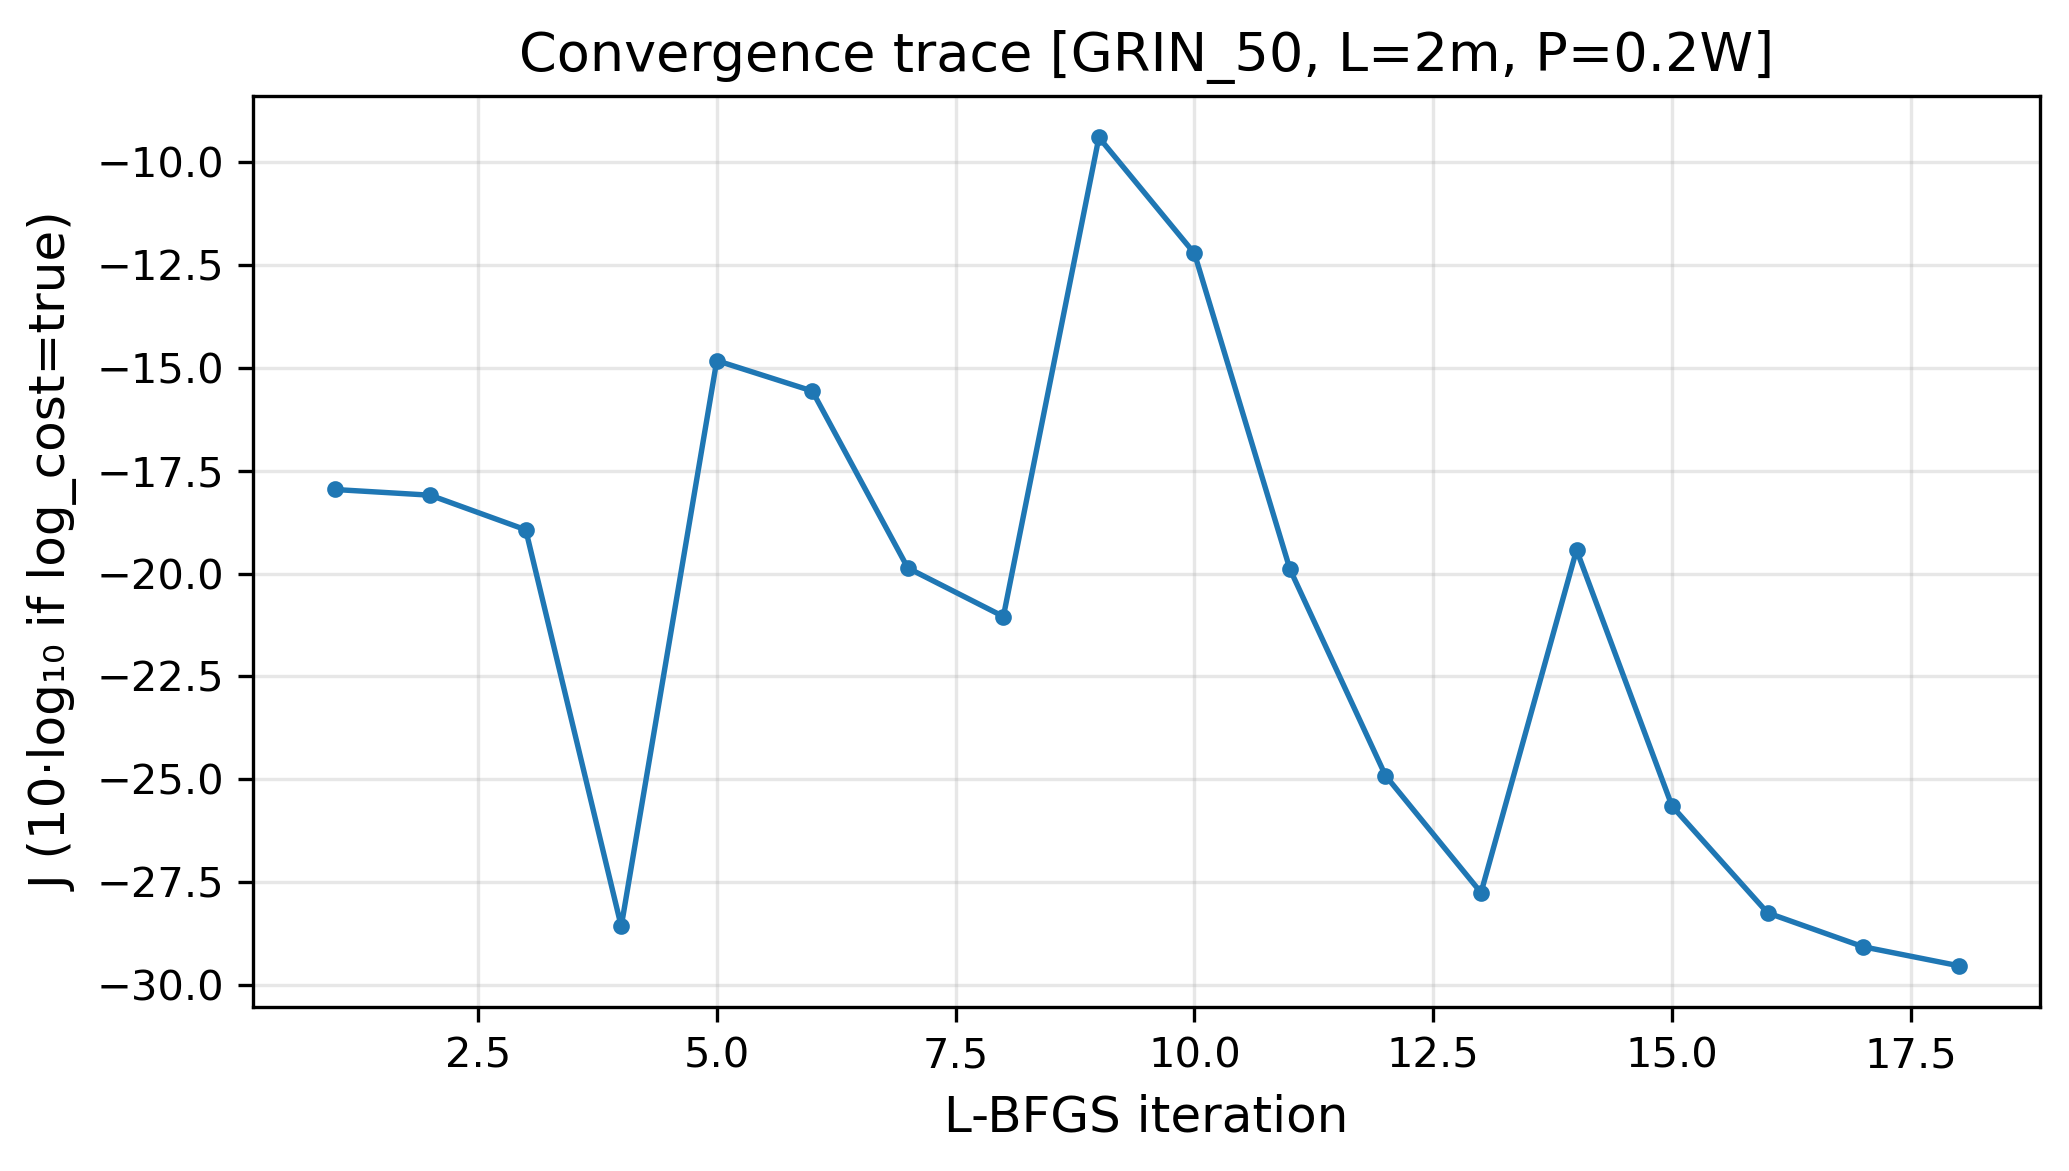
\includegraphics[width=\linewidth]{figures/mmf_accepted_convergence.png}
\caption*{Convergence trace.}
\end{minipage}
\caption{The accepted phase is still engineered and oscillatory. This is a
simulation candidate, not a lab actuator prescription.}
\end{figure}

\FloatBarrier

\section{Interpretation}

The MMF lane changed from ``blocked by invalid-window'' to ``qualified
simulation result.'' The key scientific behavior survives after the trust
correction: boundary and GDD penalties can keep the temporal window clean while
still producing large Raman suppression.

The result should be presented with discipline. It supports shared spectral
phase as a possible control mechanism in an idealized GRIN-50 MMF model. It
does not yet prove robustness to launch changes, random mode coupling, more
modes, experimental wavefront shapers, or a larger \(N_t=8192\) grid.

\section{Presentation Capsule}

If this note becomes a presentation block, the clean message is:
\begin{itemize}
    \item MMF is harder because Raman is mode-resolved and launch/coupling
    assumptions matter.
    \item The first large-gain result was rejected because the pulse touched
    the temporal window boundary.
    \item The accepted constrained run still gives a \(31.7\,\mathrm{dB}\)
    reduction and passes raw edge diagnostics.
    \item The honest claim is an idealized six-mode GRIN-50 simulation result,
    not generic experimental MMF Raman suppression.
\end{itemize}

\section{Limitations}

\begin{itemize}
    \item \textbf{No broad experimental claim.} The model is idealized and uses
    six scalar modes.
    \item \textbf{Shared spectral phase only.} This is not independent spatial
    wavefront control of each mode.
    \item \textbf{Launch sensitivity open.} Default launch is LP01-heavy; other
    launch compositions still need a matrix of checks.
    \item \textbf{Random coupling open.} The accepted result does not include a
    random or degenerate mode-coupling robustness sweep.
    \item \textbf{Grid-refinement gate open.} The \(N_t=8192\), \(96\,\mathrm{ps}\)
    refinement is currently blocked by memory/compute availability.
    \item \textbf{Phase realism open.} The accepted phase has sub-ps to roughly
    ps-scale group-delay structure and should be simplified before lab claims.
\end{itemize}

\section{Reproduction Capsule}

Planning-only front-layer check:
\begin{verbatim}
julia -t auto --project=. scripts/canonical/run_experiment.jl \
  --dry-run grin50_mmf_phase_sum_poc
\end{verbatim}

Accepted constrained candidate, to run on burst or equivalent heavy compute:
\begin{verbatim}
MMF_VALIDATION_SAVE_DIR=results/raman/mmf_validation_gdd \
MMF_VALIDATION_CASES=threshold \
MMF_VALIDATION_MAX_ITER=4 \
MMF_VALIDATION_THRESHOLD_TW=96 \
MMF_VALIDATION_THRESHOLD_NT=4096 \
MMF_VALIDATION_LAMBDA_BOUNDARY=0.05 \
MMF_VALIDATION_LAMBDA_GDD=1e-4 \
julia -t auto --project=. scripts/research/mmf/mmf_window_validation.jl
\end{verbatim}

Expected closeout:
\begin{itemize}
    \item validation summary table;
    \item phase profile and phase diagnostic;
    \item optimized and no-shaping heat maps;
    \item total and per-mode spectra;
    \item raw input/output temporal-edge fractions;
    \item explicit statement of whether the result is accepted, rejected, or
    compute-blocked.
\end{itemize}

\section{Sources}

\begin{thebibliography}{9}

\bibitem{pourbeyram2013}
H. Pourbeyram, G. P. Agrawal, and A. Mafi.
``Stimulated Raman scattering cascade spanning the wavelength range of
523 to 1750 nm using a graded-index multimode optical fiber.''
\url{https://arxiv.org/abs/1301.6203}

\bibitem{krupa2017}
K. Krupa et al.
``Spatial beam self-cleaning in multimode fibres.''
\textit{Nature Photonics}, 2017.
\url{https://doi.org/10.1038/nphoton.2017.32}

\bibitem{deliancourt2019}
E. Deliancourt et al.
``Wavefront shaping for optimized many-mode Kerr beam self-cleaning in
graded-index multimode fiber.''
\url{https://arxiv.org/abs/1902.04453}

\bibitem{sidelnikov2019}
O. Sidelnikov et al.
``Effect of random mode coupling on Kerr beam self-cleaning in graded-index
multimode fibers.''
\url{https://arxiv.org/abs/1908.07745}

\bibitem{melchert2021}
O. Melchert and A. Demircan.
``A python package for ultrashort optical pulse propagation in terms of forward
models for the analytic signal.''
\url{https://arxiv.org/abs/2104.11649}

\end{thebibliography}

\end{document}
